\documentclass[11pt]{amsart}

\setlength{\textwidth}{6in} 
\setlength{\textheight}{8.7in}
\setlength{\oddsidemargin}{.3in}
\setlength{\evensidemargin}{0.3in}
\setlength{\topmargin}{-.25in}

\usepackage{amssymb, amsfonts, amsmath, amsthm}
\usepackage{xcolor} 
 
\pagestyle{headings}

\usepackage{tikz}
\usetikzlibrary{arrows.meta, decorations.markings}


\newtheorem{theorem}{Theorem}[section]
\newtheorem{lemma}[theorem]{Lemma}
\newtheorem{proposition}[theorem]{Proposition}
\newtheorem{corollary}[theorem]{Corollary}
\newtheorem{prop-and-def}[theorem]{Proposition and Definition}

\theoremstyle{definition}
\newtheorem{definition}[theorem]{Definition}
\newtheorem{notation}[theorem]{Notation}
\newtheorem{remark}[theorem]{Remark}
\newtheorem{definition-and-remark}[theorem]{Definition and Remark}
\newtheorem{remark-and-notation}[theorem]{Remark and Notation}
\newtheorem{notation-and-remark}[theorem]{Notation and Remark}
\newtheorem{example}[theorem]{Example}
\newtheorem{problem}[theorem]{Problem}
\newtheorem{solution}[theorem]{Solution}



\numberwithin{equation}{section}


\begin{document}

\section{Review}
\begin{definition}
    A probability space is a set $\Omega$ equipped with a $\sigma$-algebra $\mathcal A$ and a probability measure $ P:\mathcal A\to[0,1]$ with $ P(\Omega)=1$.
\end{definition}
\begin{definition}
    For events, $A,B$ with $P(B)\ne 0$, define the conditional probability
    \begin{align*}
        P(A|B)=\frac{P(A\cap B)}{P(B)}
    \end{align*}
\end{definition}
\begin{definition}
    We say events $A$ and $B$ are independent when $P(A\cap B)=P(A)P(B)$. We say events $A_1,A_2,\ldots,A_n$ are independent if for any $j_1,j_2,\ldots,j_k$ with $1\le j_1<j_2<\ldots<j_k\le n$, we have that 
    \begin{align*}
        P(\bigcap_{i=1}^kA_{j_i})=\prod_{i=1}^kP(A_{j_i})
    \end{align*}
\end{definition}
\begin{definition}
    A random variable on a probability space $(\Omega,\mathcal A,P)$ is a function $X:\Omega\to\mathbb R$ such that the event $\{X\le x\}=\{s\in\Omega:X(s)\le x\}$ is an event (element of $\mathcal A$).
\end{definition}
\begin{proposition}
    For a random variable $X$ and $x\in\mathbb R$, the following are events:
    \begin{enumerate}
        \item $X<x$
        \item $X=x$
    \end{enumerate}
\end{proposition}
\begin{definition}
    A random variable $X$ is discrete when the support $\{x\in\mathbb R:P(X=x)>0\}$ is countable. Define $p:\mathbb R\to\mathbb R$ as $p(x)=P(X=x)$ (probability mass function) and $F(x)=P(X\le x)$ (cumulative distribution function). Define $\overline{F}=1-F$ (probability tail function).
\end{definition}
\begin{definition}
    A random variable $X$ is continuous when its cdf is (almost everywhere) differentiable. Define $f=F'$ to be the probability density function of $X$.
\end{definition}
\begin{definition}
    The expected value of a discrete random variable is
    \begin{align*}
        E[X]=\sum_{x}xp(x)
    \end{align*}
    The expected value of a continuous random variable is
    \begin{align*}
        E[X]=\int_{-\infty}^\infty xf(x)dx
    \end{align*}
\end{definition}
\begin{definition}
    The moment generating function $\phi_X:\mathbb R\to\mathbb R$ of a random variable $X$ is the function
    \begin{align*}
        \phi_X(t)=E[e^{tX}]
    \end{align*}
\end{definition}
\begin{proposition}
    Let $\phi_X$ be smooth in some interval $(-\delta,\delta)$ so that
    \begin{align*}
        \phi_X(t)=\sum_{k=0}^\infty\frac{a_k}{k!}t^k
    \end{align*}
    Then $a_k=E[X^k]$.
\end{proposition}
\begin{definition}
    We say random variables $X_1,X_2,\ldots,X_n$ are independent if for any $1\le a_1<\ldots<a_k\le n$, we have that 
    \begin{align*}
        P(X_{a_1}\le v_1,X_{a_2}\le v_2,\ldots,X_{a_k}=v_k)\le\prod_{j=1}^kF_{X_j}(v_j)
    \end{align*}
\end{definition}
\begin{proposition}
    Let $X,Y$ be random variables. Let $p_{XY}$ be the joint pmf of $X$ and $Y$. Then $X,Y$ are independent if and only 
    \begin{align*}
        p_{XY}(x,y)=p_X(x)p_Y(y)
    \end{align*}
    for all $x,y\in\mathbb R$.
\end{proposition}
\begin{proof}
    Fill in.
\end{proof}
\begin{proposition}
    Let $X_1,X_2$ be (continuous or discrete) independent random variables and $g,h:\mathbb R\to\mathbb R$. Then
    \begin{align*}
        E[g(X_1)h(X_2)]=E[g(X_1)]E[h(X_2)]
    \end{align*}
\end{proposition}
\begin{proof}
    For discrete random variables, we have that
    \begin{align*}
        E[g(X_1)h(X_2)]&=\sum_{(x_1,x_2)}g(x_1)h(x_2)p(x_1,x_2)\\
        &=\sum_{(x_1,x_2)}g(x_1)h(x_2)p_1(x_1)p_2(x_2)\\
        &=\sum_{x_1}\sum_{x_2}g(x_1)p_1(x_1)h(x_2)p_2(x_2)\\
        &=\sum_{x_1}g(x_1)p_1(x_1)\sum_{x_2}h(x_2)p_2(x_2)\\
        &=E[g(X_1)]E[h(X_2)]
    \end{align*}
    A similar proof for continuous random variables follows by Fubini's theorem.
\end{proof}
\begin{theorem}
    When $X_1,\ldots,X_n$ are independent random variables and $T=X_1+\ldots+X_n$, we have that $\phi_T(t)=\prod_{k=1}^n\phi_{X_k}(t)$.
\end{theorem}
\begin{proof}
    Compute:
    \begin{align*}
        \phi_T(t)&=E[e^{t(X_1+\ldots+X_n)}]\\
        &=E[e^{tX_1}\cdots e^{tX_n}]\\
        &=E[e^{tX_1}]\cdots E[e^{tX_n}]\\
        &=\phi_{X_1}(t)\cdots\phi_{X_n}(t)
    \end{align*}
\end{proof}
\begin{definition}
    Let $X$ be a random variable and $\{X_n\}_{n=1}^\infty$ be a sequence of random variables. 
    \begin{enumerate}
        \item We say $X_n\to X$ in distribution if
        \begin{align*}
            \lim_{n\to\infty}P(X_n\le X)=P(X\le x)
        \end{align*}
        whenever $F_X$ is continuous at $x$.
        \item We say $X_n\to X$ in probability if
        \begin{align*}
            \lim_{n\to\infty}P(|X_n-X|\ge\varepsilon)=0
        \end{align*}
        for all $\varepsilon>0$.
        \item We say $X_n\to X$ almost surely (a.s.) if 
        \begin{align*}
            P(\lim_{n\to\infty}X_n=X)=1
        \end{align*}
    \end{enumerate}
\end{definition}
\begin{proposition}
    In the previous definition, $(3)\implies(2)\implies(1)$.
\end{proposition}
\begin{proof}
    $(3)\implies(2)$:

    Remark that if $X_n\to X$ almost surely, then for $\varepsilon>0$, then for $\varepsilon>0$, the probability all but finitely many $X_n$ satisfy $|X_n-X|\ge\varepsilon$ is 0. In other words,
    \begin{align*}
        0&=P(\limsup_n |X_n-X|\ge\varepsilon)\\
        &\ge \limsup_nP(|X_n-X|\ge\varepsilon)\\
    \end{align*}
    which automatically gives us that $\displaystyle\lim_{n\to\infty}P(|X_n-X|\ge\varepsilon)=0$

    $(2)\implies(1)$:

    We first remark that for random variables $X,Y$, we have that
    \begin{align*}
        P(X\le x)\le P(Y\le x+\varepsilon)+P(|Y-X|>\varepsilon)
    \end{align*}
    since whenever $X\le x$, either $Y\le x+\varepsilon$ or $Y>x+\varepsilon$, in which case $|Y-X|>\varepsilon$.

    We now prove that for $\varepsilon>0$, we have that
    \begin{align*}
        P(X\le a-\varepsilon)\le\lim_{n\to\infty} P(X_n\le a)\le P(X\le a+\varepsilon)
    \end{align*}
    Note that $P(X_n\le a)\le P(X\le a+\varepsilon)+P(|X-X_n|>\varepsilon)$. Taking $n\to\infty$, we get that $\displaystyle\lim_{n\to\infty}P(X_n\le a)\le P(X\le a+\varepsilon)$.

    Similarly, $P(X\le a-\varepsilon)\le P(X_n\le a)+P(|X_n-X|>\varepsilon)$. Taking $n\to\infty$ gives the desired inequality again.

    Finally, taking $\varepsilon\to0^+$ gives the desired result.
\end{proof}
\begin{lemma}[Chebyshev's inequality]
    Let $X$ be a random variable with finite variance non-zero variance. Then for any real number $k>0$, 
    \begin{align*}
        P(|X-\mu|\ge k\sigma)\le\frac{1}{k^2}
    \end{align*}
\end{lemma}
\begin{theorem}[Weak Law of Large Numbers]
\label{wll}
    If $X_1,X_2,\ldots$ is an i.i.d. sequence of random variables with common mean $\mu$ and $E[|X_1|]<\infty$, then
    \begin{align*}
        \overline{X}_n=\frac{X_1+\ldots+X_n}{n}\to\mu
    \end{align*}
    in probability as $n\to\infty$.
\end{theorem}
\begin{proof}
    We prove the case where $X_1$ has finite variance.
    
    Let $\sigma=SD(X_1)$ and $\sigma_n=SD(\overline{X}_n)$. We compute:
    \begin{align*}
        \sigma_n^2&=Var(\overline{X}_n)\\
        &=Var(\frac{1}{n}\sum_{k=1}^nX_k)\\
        &=\frac{1}{n^2}Var(\sum_{k=1}^nX_k)\\
        &=\frac{1}{n^2}\sum_{k=1}^nVar(X_k)\\
        &=\frac{\sigma^2}{n}
    \end{align*}
    Also note that $E[\overline{X}_n]=\mu$.
    
    Now by Chebyshev's inequality, we have that
    \begin{align*}
        P(|\overline{X}_n-\mu|\ge \frac{k\sigma}{\sqrt{n}})\le\frac{1}{k^2}
    \end{align*}
    for $k>0$. Set $k=\frac{\sqrt{n}\varepsilon}{\sigma}$ yields that
    \begin{align*}
        P(|\overline{X}_n-\mu|\ge \varepsilon)\le\frac{\sigma^2}{n}
    \end{align*}
    Taking $n\to\infty$ yields the desired result.
\end{proof}
\begin{theorem}[Strong Law of Large Numbers]
    The convergence in \ref{wll} is a.s.
\end{theorem}
We omit a proof of this theorem.
\section{Conditional Distributions and Conditional Expectation}
\begin{definition}
    If $X_1$ and $X_2$ are discrete random variables with joint pmf $p(x_1,x_2)$ and marginal pmfs $p_1(x_1)$ and $p_2(x_2)$, then the conditional distribution of $X_1$ given $X_2=x_2$, denoted $X_1|(X_2=x_2)$, is defined as
    \begin{align*}
        p_{1|2}(x_1|x_2)=\frac{P(X_1=x_1\text{ and }X_2=x_2)}{P(X_2=x_2)}=\frac{p(x_1,x_2)}{p_2(x_2)}
    \end{align*}
    A similar definition holds for $p_{2|1}$.
\end{definition}
\begin{remark}
    When $X_1$ and $X_2$ are independent, $p(x_1,x_2)=p_1(x_1)p_2(x_2)$ so that 
    \begin{align*}
        p_{1|2}(x_1|x_2)=p_1(x_1)
    \end{align*}
\end{remark}
\begin{definition}
    The conditional mean of $X_1|(X_2=x_2)$ is 
    \begin{align*}
        E[X_1|X_2=x_2]=\sum_{x_1}x_1p_{1|2}(x_1|x_2)
    \end{align*}
\end{definition}
\begin{definition}
    The conditional variance of $X_1|(X_2=x_2)$ is
    \begin{align*}
        Var(X_1|X_2=x_2)=E[(X_1-E[X_1|X_2=x_2])^2|X_2=x_2]
    \end{align*}
\end{definition}
\begin{theorem}
    $\displaystyle Var(X_1|X_2=x_2)=E[X_1^2|X_2=x_2]-E[X_1|X_2=x_2]^2$
\end{theorem}
\begin{proof}
    Compute:
    \begin{align*}
        Var(X_1|X_2=x_2)&=E[(X_1-E[X_1|X_2=x_2])^2|X_2=x_2]\\
        &=E[X_1^2-2X_1E[X_1|X_2=x_2]+E[X_1|X_2=x_2]^2|X_2=x_2]\\
        &=E[X_1^2|X_2=x_2]-2[X_1|X_2=x_2]E[X_1|X_2=x_2]+E[X_1|X_2=x_2]^2\\
        &=E[X_1^2|X_2=x_2]-E[X_1|X_2=x_2]^2
    \end{align*}
\end{proof}
\begin{example}
    Let $X_i\sim\mathrm{BIN}(n_i,p)$ for $i=1,2$ be independent. Find the distribution of $X_1$ given that $X_1+X_2=m$.
\end{example}
\addtocounter{theorem}{-1}
\begin{solution}
    We are trying to find $P(X_1=t|X_1+X_2=m)$. Compute:
    \begin{align*}
        P(X_1=t|X_1+X_2=m)&=\frac{P(X_1=t,X_2=m-t)}{P(X_1+X_2=m)}\\
        &=\frac{P(X_1=t)P(X_2=m-t)}{P(X_1+X_2=m)}
    \end{align*}
    Now note that $X_1+X_2$ is distributed $\mathrm{BIN}(n_1+n_2,p)$ so we may plug everything in and get
    \begin{align*}
        \frac{P(X_1=t)P(X_2=m-t)}{P(X_1+X_2=m)}&=\frac{\binom{n_1}{t}p^t(1-p)^{n_1-t}\binom{n_2}{m-t}p^{m-t}(1-p)^{n_2-m+t}}{\binom{n_1+n_2}{m}p^m(1-p)^{n_1+n_2-m}}\\
        &=\frac{\binom{n_1}{t}\binom{n_2}{m-t}}{\binom{n_1+n_2}{m}}
    \end{align*}
    which is $\mathrm{HG}(n_1+n_2,n_1,m)$
\end{solution}
\begin{example}
    Let $X_1,X_2,\ldots,X_m$ be independent with $X_i\sim\mathrm{POI}(\lambda_i)$ for $i=1,\ldots,m$. Find the conditional distribution of $X_j|(\sum_iX_i=n)$.
\end{example}
\addtocounter{theorem}{-1}
\begin{solution}
    Compute:
    \begin{align*}
        P(X_j=t|\sum_{i}X_i=n)&=\frac{P(X_j=t,\sum_{i}X_i=n)}{P(\sum_iX_i=n)}\\
        &=\frac{P(X_j=t,\sum_{i\ne j}X_i=n-t)}{P(\sum_iX_i=n)}\\
        &=\frac{\sum_{\sum_{j\ne i}x_j=n-t}P(X_j=t,X_i=x_i\text{ for }i\ne j)}{P(\sum_iX_i=n)}\\
        &=P(x_j=t)\frac{P(\sum_{i\ne j}X_i=n-t}{P(\sum_iX_i=n)}\\
        &=\frac{e^{-\lambda_j}\lambda_j^t}{t!}\cdot\frac{e^{-\sum_{i\ne j}\lambda_i}(\sum_{i\ne j}\lambda_i)^{n-t}}{(n-t)!}\frac{n!}{e^{-\sum_i\lambda_i}(\sum_i\lambda_i)^n}
    \end{align*}
    Setting $\lambda=\sum_i\lambda_i$ gives
    \begin{align*}
        \frac{e^{-\lambda_j}\lambda_j^t}{t!}\cdot\frac{e^{-\sum_{i\ne j}\lambda_i}(\sum_{i\ne j}\lambda_i)^{n-t}}{(n-t)!}\frac{n!}{e^{-\sum_i\lambda_i}(\sum_i\lambda_i)^n}&=\frac{n!}{t!(n-t)!}\cdot\frac{\lambda_j^t(\lambda-\lambda_j)^{n-t}}{\lambda^n}\\
        &=\binom{n}{t}\left(\frac{\lambda_j}{\lambda}\right)^t\left(1-\frac{\lambda_j}{\lambda}\right)^{n-t}
    \end{align*}
    which is $\mathrm{BIN}(n,\frac{\lambda_j}{\lambda})$
\end{solution}
\begin{definition}
    For jointly continuous random variables $X$ and $Y$, we define
    \begin{align*}
        f_Y(y)=\lim_{dy\to0^+}\frac{P(y\le Y\le y+dy)}{dy}
    \end{align*}
    to be the pdf for $Y$.
\end{definition}
\begin{definition}
    We define the joint pdf for jointly continuous random variables $X,Y$ to be
    \begin{align*}
        f(x,y)=\lim_{(dx,dy)\to(0,0)}\frac{P(x\le X\le x+dx,y\le Y\le y+dy)}{dxdy}
    \end{align*}
\end{definition}
\begin{remark}
    For small values of $dx,dy$, we have that
    \begin{align*}
        P(x\le X\le x+dx|y\le Y\le y+dy)&=\frac{P(x\le X\le x+dx,y\le Y\le y+dy)}{P(y\le Y\le y+dy)}\\
        &\approx\frac{f(x,y)dxdy}{f_Y(y)dy}\\
        &=\frac{f(x,y)dx}{f_Y(y)}
    \end{align*}
    This yields the following definition:
\end{remark}
\begin{definition}
    The conditional pdf of $X$ given $Y=y$ is given by
    \begin{align*}
        f_{X|Y}(x|y)=\frac{f(x,y)}{f_Y(y)}
    \end{align*}
 \end{definition}
 \begin{example}
     Suppose the joint pdf of $X$ and $Y$ is given by
     \begin{align*}
         f(x,y)=\begin{cases}
             5e^{-3x-y}, & 0<2x<y<\infty\\
             0, &\text{otherwise}
         \end{cases}
     \end{align*}
     Determine the conditional distribution of $Y|(X=x)$ for $0<x<\infty$.
 \end{example}
 \addtocounter{theorem}{-1}
 \begin{solution}
     We compute $f_X(x)$.
     \begin{align*}
         f_X(x)&=\int_{2x}^\infty5e^{-3x-y}dy\\
         &=5e^{-3x}\int_{2x}^\infty e^{-y}dy\\
         &=5e^{-3x}[-e^{-y}]^\infty_{2x}\\
         &=5e^{-5x}
     \end{align*}
     This yields that 
     \begin{align*}
         f_{Y|X}(y|x)&=\frac{f(x,y)}{5e^{-5x}}\\
         &=\frac{5e^{-3x-y}}{5e^{-5x}}\\
         &=\frac{e^{-y}}{e^{-2x}}\\
         &=e^{2x-y}
     \end{align*}
     whenever $y>2x$.
 \end{solution}
 \begin{definition}
     If $X$ and $Y$ are jointly continuous random variables and $g:\mathbb R\to\mathbb R$, then the conditional expectation of $g(X)$ given $Y=y$ is given by
     \begin{align*}
         E[g(X)|Y=y]=\int_{-\infty}^\infty g(x)f_{X|Y}(x|y)dx
     \end{align*}
 \end{definition}
 \begin{definition}
     The conditional variance of $X|Y=y$ is defined to be the variance of the distribution generated by $X|Y=y$.
 \end{definition}
 \begin{remark}
     Suppose we had $X$ a continuous rv and $Y$ a discrete rv. We can define the joint probability function to be
     \begin{align*}
         f(x,y)=\lim_{dx\to0}\frac{P(x\le X\le x+dx,Y=y)}{dx}
     \end{align*}
     To define conditional probability $f_{X|Y}$, we note that the following should hold:
     \begin{align*}
         f_{X|Y}(x|y)&=\lim_{dx\to0}\frac{P(x\le X\le x+dx|Y=y)}{dx}\\
         &=\lim_{dx\to0}\frac{P(Y=y|x\le X\le x+dx)}{p_Y(y)}\cdot\frac{P(x\le X\le x+dx)}{dx}\\
         &=\frac{p(y|x)}{p_Y(y)}f_X(x)
     \end{align*}
     where $p_{Y|X}(y|x)=P(Y=y|X=x)$. 
 \end{remark}
 \begin{example}
     Suppose $X\sim U(0,1)$ and $Y|(X=x)\sim\mathrm{BERN}(x)$. Find the conditional distribution $X|(Y=y)$.
 \end{example}
 \addtocounter{theorem}{-1}
 \begin{solution}
     Note that 
     \begin{align*}
         p_Y(y)&=\int_{0}^1 f(y|x)f_X(x)dx\\
         &=\int_{0}^1 (yx+(1-y)(1-x))dx\\
         &=\left[\frac{1}{2}yx^2+(1-y)x-\frac{1}{2}(1-y)x^2\right]^{1}_{0}\\
         &=\frac{1}{2}y+(1-y)-\frac{1}{2}(1-y)\\
         &=\frac{1}{2}
     \end{align*}
     By definition,
     \begin{align*}
         f_{X|Y}(x|y)&=\frac{p(y|x)}{p_Y(y)}f_X(x)\\
         &=\frac{yx+(1-y)(1-x)}{\frac{1}{2}}\\
         &=2(yx+(1-y)(1-x))
     \end{align*}
 \end{solution}
 \begin{remark}
     For a function $g:\mathbb R\to\mathbb R$, and random variable $X$ and $Y$, note that
     \begin{align*}
         E[g(X)|Y=y]
     \end{align*}
     is a function of $y$, say $v(y)=E[g(X)|Y=y]$. We remark that $v(Y)$ is a random variable. In fact, the following theorem about $v$ holds:
 \end{remark}
 \begin{theorem}[Law of total expectation]
     For random variables $X$ and $Y$,
     \begin{align*}
         E[g(X)]=E[v(Y)]=E[E[g(X)|Y]]
     \end{align*}
 \end{theorem}
 \begin{proof}
     When $Y$ has probability function $f_Y$ (for discrete or continuous), we have that
     \begin{align*}
         E[E[g(X)|Y]]&=\int_yE[g(X)|Y=y]f_Y(y)\\
         &=\int_{y}\int_xg(x)f_{X|Y}(x|y)f_Y(y)\\
         &=\int_xg(x)\int_yf_{X|Y}(x|y)f_Y(y)\\
         &=\int_xg(x)f_X(x)\\
         &=E[g(X)]
     \end{align*}
 \end{proof}
 \begin{example}
     Suppose $X\sim\mathrm{GEO}_t(p)$ with pmf $p_X(x)=(1-p)^{x-1}p$ for $x=1,2,\ldots$. Compute $E[X]$ and $Var(X)$.

     Let $Y$ be defined by $Y=\begin{cases}
         1, & X=1\\
         0, & \text{otherwise}
     \end{cases}$. We note that $E[X|Y=1]=1$ and that
     \begin{align*}
         p_{X|Y}(x|0)&=P(X=x|Y=0)\\
         &=P(X=x|X>1)\\
         &=\frac{P(X=x,X>1)}{P(X>1)}\\
         &=\frac{(1-p)^{x-1}p}{(1-p)}\\
         &=(1-p)^{x-2}p\\
         &=p_X(x-1)
     \end{align*}
     for $x\ge 2$ so that $X|(Y=0)$ is distributed the same as $X+1$ and thus $E[X|Y=0]=E[X]+1$. Furthermore, we note that $Y\sim\mathrm{BERN}(p)$. This yields that 
     \begin{align*}
         E[X]&=p_Y(1)+(E[X]+1)p_Y(0)\\
         &=p+(E[X]+1)(1-p)\\
         &=p+(1-p)E[X]+1-p\\
         &=1+(1-p)E[X]
     \end{align*}
     which yields that $E[X]=\frac{1}{p}$.

     In order to compute the variance, note that we are just doing the same calculation on $E[X^2]$. We get that $E[X^2|Y=1]=1$ and that
     \begin{align*}
         p_{X^2|Y}(x^2|0)&=P(X^2=x^2|Y=0)\\
         &=P(X=x|Y=0)\\
         &=p_X(x-1)\\
         &=p_{X^2}((x-1)^2)
     \end{align*}
     so that $X^2|(Y=0)$ is distributed identically to $(X+1)^2$ and thus 
     \begin{align*}
         E[X^2|Y=1]=E[(X+1)^2]=E[X^2]+2E[X]+1
     \end{align*}
     This yields that 
     \begin{align*}
         E[X^2]&=p+(E[X^2]+2E[X]+1)(1-p)\\
         &=p+(1-p)E[X^2]+(1-p)\frac{2}{p}+(1-p)
     \end{align*}
     In other words,
     \begin{align*}
         pE[X^2]&=p+\frac{2}{p}-2+1-p\\
         &=\frac{2}{p}-1
     \end{align*}
     so that $E[X^2]=\frac{2}{p^2}-\frac{1}{p}$ and 
     \begin{align*}
         Var(X)=E[X^2]-E[X]^2&=\frac{2}{p^2}-\frac{1}{p}-\frac{1}{p^2}\\
         &=\frac{1}{p^2}-\frac{1}{p}
     \end{align*}
 \end{example}
 \begin{theorem}
     For rvs $X$ and $Y$,
     \begin{align*}
         Var(X)=E[Var(X|Y)]+Var(E[X|Y])
     \end{align*}
 \end{theorem}
 \begin{proof}
    Note that 
    \begin{align*}
        E[Var(X|Y)]&=E[E[X^2|Y]-E[X|Y]^2]\\
        &=E[E[X^2|Y]]-E[E[X|Y]^2]\\
        &=E[X^2]-E[E[X|Y]^2]
    \end{align*}
    and that
    \begin{align*}
        Var(E[X|Y])&=E[E[X|Y]^2]-E[E[X|Y]]^2\\
        &=E[E[X|Y]^2]-E[X]^2
    \end{align*}
    Adding the two together cancels out the $E[E[X|Y]^2]$ term and we are left with $E[X^2]-E[X]^2$, as desired.
 \end{proof}
 \begin{example}[Random Sum]\label{randomsum}
     Suppose $\{X_i\}$ is a sequence of iid rvs with common mean $\mu$ and common variance $\sigma^2$. Let $N$ be a discrete, nonnegative random variable independent of the $X_i$'s. Find the mean and variance of $T=\sum_{i=1}^NX_i$.
 \end{example}
 \addtocounter{theorem}{-1}
 \begin{solution}
     Note that
     \begin{align*}
         E[T|N=n]&=E[\sum_{i=1}^NX_i|N=n]\\
         &=E[\sum_{i=1}^nX_i|N=n]\\
         &=\sum_{i=1}^nE[X_i|N=n]\\
         &=n\mu
     \end{align*}
     so that 
     \begin{align*}
         E[T]&=E[E[T|N]]\\
         &=\sum_{n=0}^\infty p_N(n)E[T|N=n]\\
         &=\sum_{n=0}^\infty n\mu p_N(n)\\
         &=\mu\sum_{n=0}^\infty np_N(n)\\
         &=\mu E[N]
     \end{align*}
     To compute the variance, note that
     \begin{align*}
         Var(T|N=n)&=Var(\sum_{i=1}^nX_i|N=n)\\
         &=\sum_{i=1}^nVar(X_i|N=n)\\
         &=\sum_{i=1}^nVar(X_i)\\
         &=n\sigma^2
     \end{align*}
     so that
     \begin{align*}
         Var(T)&=E[Var(T|N)]+Var(E[T|N])\\
         &=E[N\sigma^2]+Var(N\mu)\\
         &=\sigma^2E[N]+\mu^2Var(N)
     \end{align*}
 \end{solution}
 \begin{remark}
     Let $A$ be some event of interest and define a random variable $X$ by
     \begin{align*}
         X(s)=\begin{cases}
             1, & s\in A\\
             0, & s\not\in A
         \end{cases}
     \end{align*}
     so that $P(X=1)=P(A)$ and $P(X=0)=P(A^c)=1-P(A)$ and we get $X\sim\mathrm{BERN}(P(A))$. We also see that $P(A)=E[X]$. For a random variable $Y$, we get that $E[X]=E[E[X|Y]]$ and
     \begin{align*}
        E[X|Y=y]=p_{X|Y}(1|y)=P(A|Y=y)
     \end{align*}
     Which implies that
     \begin{align*}
         P(A)=E[X]=E[E[X|Y]]=\begin{cases}
             \sum_{y}p_Y(y)P(A|Y=y), & Y\text{ discrete}\\
             \int_{-\infty}^\infty f_Y(y)P(A|Y=y)dy, & Y\text{ continuous}
         \end{cases}
     \end{align*}
     which is the law of total probability.
 \end{remark}
 \begin{example}
     Suppose $X,Y$ continuous independent random variables. Find an expression for $P(X<Y)$.
 \end{example}
 \addtocounter{theorem}{-1}
 \begin{solution}
     Let $A$ be the event that $X<Y$. Define $Z$ to be the indicator random variable of $A$. We note that 
     \begin{align*}
         P(A|Y=y)&=P(X<Y|Y=y)\\
         &=P(X<y|Y=y)\\
         &=F_X(y)
     \end{align*}
     so that
     \begin{align*}
         P(A)=\int_{-\infty}^\infty F_X(y)f_Y(y)dy
     \end{align*}
 \end{solution}
 \begin{remark}
     When $X$ and $Y$ are iid, the above simplifies to
     \begin{align*}
         \int_{-\infty}^\infty F_X(y)f_X(y)dy
     \end{align*}
     Note that the probability that $X=Y$ is 0 and that the probability that $X>Y$ is the same as the probability that $X<Y$ by the same computation. As such, the integral above evaluates to $\frac{1}{2}$.

     Alternatively, we may make the substitution $u=F_X(y)$ and $du=f_X(y)dy$ so that
     \begin{align*}
         \int_{-\infty}^\infty F_X(y)f_X(y)dy&=\int_0^1udu\\
         &=\frac{1}{2}
     \end{align*}
 \end{remark}
 \begin{example}\label{expex}
     Suppose $X\sim\mathrm{EXP}(\lambda_1)$ and $Y\sim\mathrm{EXP}(\lambda_2)$. Show that
     \begin{align*}
         P(X<Y)=\frac{\lambda_1}{\lambda_1+\lambda_2}
     \end{align*}
     Plug and chug:
     \begin{align*}
         F_X(y)=1-e^{-\lambda_1 x}\\
         f_Y(y)=\lambda_2e^{-\lambda_2 x}
     \end{align*}
     Putting these two into the formula yields
     \begin{align*}
         P(X<Y)&=\int_{0}^{\infty}(1-e^{-\lambda_1 y})\lambda_2e^{-\lambda_2 y}dy\\
         &=\lambda_2\int_0^\infty e^{-\lambda_2 y}dy-\lambda_2\int_0^\infty e^{-(\lambda_1+\lambda_2)y}dy\\
         &=1-\frac{\lambda_2}{\lambda_1+\lambda_2}\\
         &=\frac{\lambda_1}{\lambda_1+\lambda_2}
     \end{align*}
 \end{example}
 \begin{example}
     Let $W,X,Y$ be independent continuous rvs on $(0,\infty)$. If $Z=X|(X<Y)$, then show that $(W,X)|(W<X<Y)$ and $(W,Z)|(W<Z)$ are identically distributed.
 \end{example}
 \addtocounter{theorem}{-1}
 \begin{solution}
     Let $G(w,x)$ be the joint cdf of $(W,X)|(W<X<Y)$ so that
     \begin{align*}
         G(w,x)&=P(W\le w, X\le x|W<X<Y)\\
         &=\frac{P(W\le w, X\le x, W<X, X<Y)}{P(W<X, X<Y)}\\
     \end{align*}
     Conditioning on $X$, we see that
     \begin{align*}
         P(W<X,X<Y)&=\int_0^\infty P(W<t, t<Y|X=t)f_X(t)dt\\
         &=\int_0^\infty P(W<t, t<Y)f_X(t)dt\\
         &=\int_0^\infty P(W<t)P(t<Y)f_X(t)dt\\
         &=\int_0^\infty F_W(t)\overline{F}_Y(t)f_X(t)dt
     \end{align*}
     and we also see that
     \begin{align*}
         P(W\le w, X\le x, W<X, X<Y)&=\int_0^\infty P(W\le w, t\le x, W<t, t< Y|X=t)f_X(t)dt\\
         &=\int_0^x P(W\le w, W<t, t<Y)f_X(t)dt\\
         &=\int_0^x P(W\le w, W<t)P(t<Y)f_X(t)dt\\
         &=\int_0^x F_W(\min\{w,t\})\overline{F}_Y(t)f_X(t)dt
     \end{align*}
     We look at the cdf of $Z$:
     \begin{align*}
         F_Z(z)&=P(X\le z|X<Y)\\
         &=\frac{P(X\le z, X<Y)}{P(X<Y)}
     \end{align*}
     Conditioning on $X$ yields
     \begin{align*}
         F_Z(z)&=\frac{\int_0^\infty P(t\le x, t<Y|X=t)f_X(t)dt}{P(X<Y)}\\
         &=\frac{\int_0^zP(t<Y)f_X(t)dt}{P(X<Y)}\\
         &=\frac{\int_0^z\overline{F}_Y(t)f_X(t)dt}{P(X<Y)}
     \end{align*}
     and we get that the pdf of $Z$ is
     \begin{align*}
         f_Z(z)=\frac{1}{P(X<Y)}\overline{F}_Y(z)f_X(z)
     \end{align*}
     by the fundamental theorem.

     Now we find $P(W<Z)$ by conditioning on $Z$. This yields
     \begin{align*}
         \int_0^\infty P(W<t|Z=t)f_Z(t)dt&=\int_0^\infty P(W<t)f_Z(t)dt\\
         &=\frac{1}{P(X<Y)}\int_0^\infty f_W(t)\overline{F}_Y(t)f_X(t)dt\\
         &=\frac{P(W<X, X<Y)}{P(X<Y)}\\
     \end{align*}
     Finally, we find $P(W\le w, Z\le z|W<Z)$ by conditioning on $Z$. Note that this is equal to $\displaystyle\frac{P(W\le w, Z\le z, W<Z)}{P(W<Z)}$ and we only need to find $P(W\le w, Z\le z, W<Z)$.
     \begin{align*}
         P(W\le w, Z\le z, W<Z)&=\int_0^\infty P(W\le w, t\le z, W<t|Z=t)f_Z(t)dt\\
         &=\int_0^z P(W\le w, W<t)f_Z(t)dt\\
         &=\frac{1}{P(X<Y)}\int_0^z F_W(\min\{w,t\})\overline{F}_Y(t)f_X(t)dt
     \end{align*}
     So we finally get that
     \begin{align*}
         P(W\le w, Z\le z|W<Z)&=\frac{\frac{1}{P(X<Y)}\int_0^zF_W(\min\{w,t\})\overline{F}_Y(t)f_X(t)dt}{\frac{1}{P(X<Y)}P(W<X, X<Y)}\\
         &=\frac{P(W\le w, X\le x, W<X, X<Y)}{P(W<X, X<Y)}\\
         &=P(W\le w, X\le x|W<X<Y)\\
         &=G(w, x)
     \end{align*}
     as desired.
 \end{solution}
 \begin{remark}
     What the fuck was that?

     The idea is to expand each conditional probability and condition on some variable to obtain a simplified expression on the numerator. Then everything cancels somehow.
 \end{remark}
 \begin{remark}
     Recall from the law of total expectation, 
     \begin{align*}
         E[g(X)]=E[E[g(X)|Y]]
     \end{align*}
     For discrete $Y$, we get that
     \begin{align*}
         E[g(X)]=\sum_{y}E[g(X)|Y=y]p_Y(y)
     \end{align*}
     and for continuous $Y$, this is
     \begin{align*}
         E[g(X)]=\int_{\infty}^\infty E[g(X)|Y=y]f_Y(y)
     \end{align*}
     By a similar reasoning, for a random variable $X$ and random variables $Y_1, Y_2,\ldots,Y_n$, we see that
     \begin{align*}
         E[X|Y_j=y_j, j=1,\ldots,n]
     \end{align*}
     is a function of $y_1,\ldots,y_n$.
 \end{remark}
 \begin{example}
     Consider an experiment in which independent trials with success rate $p\in(0,1)$ are performed until $k$ consecutive successes are achieved. Determine the expected number of trials needed to achieve $k$ consecutive successes.

     For instance, when $n=2$, we get that 
     \begin{align*}
         E[]
     \end{align*}
 \end{example}
 \addtocounter{theorem}{-1}
 \begin{solution}
     Let $N_k$ be the number of trials needed to get $k$ consecutive successes.

     Remark that $N_1\sim\mathrm{GEO}_t(p)$, which has expected value $E[N_1]=\frac{1}{p}$.

     Now assume that we know $E[N_k]$. We will find $E[N_{k+1}]$. We try to use the law of total expectation on $E[N_{k+1}]$ by conditioning on the random variable
     \begin{align*}
         W=\begin{cases}
             1, & \text{if the first trial is a success}\\
             0, & \text{otherwise}
         \end{cases}
     \end{align*}
     This will yield
     \begin{align*}
         E[N_{k}]&=E[E[N_{k}|W]]\\
         &=(1-p)E[N_k|W=0]+pE[N_k|W=1]
     \end{align*}
     Remark that $N_k|(W=0)\sim N_k+1$. We would like to find a way to compute $E[N_k|W=1]$.

     However, this is really hard - note that either we get $k-1$ successes in a row or we are reduced back to the case where we must find $E[N_k]$.

     Instead, we condition on $N_{k-1}$.
     \begin{align*}
         E[N_k]&=E[E[N_k|N_{k-1}]]\\
     \end{align*}
     We define $Y|N_{k-1}=n$ by being $1$ if the $(n+1)$th trial is a success and 0 otherwise. Remark that $Y|(N_{k-1}=n)$ is distributed by $\mathrm{BERN}(p)$.

     We will try to compute $E[N_k|{N_{k-1}=n}]$ by conditioning over $y$.
     \begin{align*}
         E[N_k|N_{k-1}=n]&=E[N_k|N_{k-1}=n, Y=1]P(Y=1)+E[N_k|N_{k-1}=n, Y=0]P(Y=0)
     \end{align*}
     Note that $N_k|(N_{k-1}=n, Y=0)$ is distributed the same as $N_k+n+1$. As such, we get
     \begin{align*}
         E[N_k|N_{k-1}=n]&=(n+1)p+(n+1+E[N_k])(1-p)\\
         &=(p+1-p)(n+1)+(1-p)E[N_k]
     \end{align*}
     so that $E[N_k|N_{k-1}]=(N_{k-1}+1)+(1-p)E[N_k]$ and
     \begin{align*}
         E[N_k]&=
         E[E[N_k|N_{k-1}]]\\
         &=E[N_{k-1}+1+(1-p)E[N_k]]\\
         &=1+E[N_{k-1}]+(1-p)E[N_k]
     \end{align*}
     and we get that
     \begin{align*}
         E[N_k]=\frac{1+E[N_{k-1}]}{p}
     \end{align*}
     which is a recursive solution.

     We note that if $E[N_k]=\sum_{j=1}^k\frac{1}{p^j}$, then $E[N_{k+1}]=\frac{1}{p}+\frac{1}{p}\sum_{j=1}^k\frac{1}{p^j}=\sum_{j=1}^{k+1}\frac{1}{p^j}$, which we may simplify to
     \begin{align*}
         E[N_k]=\frac{p^{-k}-1}{1-p}
     \end{align*}
 \end{solution}
 \section{Discrete time Markov chains}
 \begin{definition}
     A stochastic process is a collection of random variables indexed by a set $\mathcal T$. We often write
     \begin{align*}
         \{X(t):t\in\mathcal T\}
     \end{align*}
     In this course, we will only consider the case when $\mathcal T$ is countable (e.g. $\mathbb N$). In this case, we may simply write
     \begin{align*}
         \{X_n:n\in\mathbb N\}
     \end{align*}
 \end{definition}
 \begin{definition}
     A stochastic process $\{X_n:n\in\mathbb N\}$ is said to be a discrete-time Markov chain (DTMC) if the following hold:
     \begin{enumerate}
         \item [(a)] $X_n$ is a discrete random variable for each $n\in\mathbb N$
         \item [(b)] For all $n\in\mathbb N$ and all states $x_0,\ldots,x_{n+1}\in\mathcal S$, the Markov property must hold:
         \begin{align*}
             P(X_{n+1}=x_{n+1}|X_n=x_n,X_{n-1}=x_{n-1},\ldots,X_0=x_0)=P(X_{n+1}=x_{n+1}|X_n=x_n)
         \end{align*}
     \end{enumerate}
 \end{definition}
 \begin{remark}
     Suppose we wish to calculate
     \begin{align*}
         P(X_{n+1}=x_{n+1}|X_n=x_n,X_{n-2}=x_{n-2},\ldots,X_0=x_0)
     \end{align*}
     By definition, this is equal to 
     \begin{align*}
         \frac{P(X_j=x_j:j=1,\ldots,n-2,n,n+1)}{P(X_j=x_j:j=1,\ldots,n-2,n)}
     \end{align*}
     Now remark that
     \begin{align*}
         &P(X_{n+1}=x_{n+1},X_n=x_n,X_j=x_j:j=0,\ldots,n-2)\\
         &=\sum_{x_{n-1}=0}^\infty P(X_j=x_j:j=1,\ldots,n+1)\\
         &=\sum_{x_{n-1}=0}^\infty P(X_{n+1}=x_{n+1}|X_j=x_j:j=1,\ldots,n)P(X_j=x_j:j=1,\ldots,n)\\
         &=\sum_{x_{n-1}=0}^\infty P(X_{n+1}=x_{n+1}|X_n=x_n)P(X_j=x_j:j=1,\ldots,n)\\
         &=P(X_{n+1}=x_{n+1}|X_n=x_n)\sum_{x_{n-1}=0}^\infty P(X_j=x_j:j=1,\ldots,n)\\
         &=P(X_{n+1}=x_{n+1}|X_n=x_n)P(X_j=x_j:j=1,\ldots,n-2,n)
     \end{align*}
     so that
     \begin{align*}
         P(X_{n+1}=x_{n+1}|X_n=x_n,X_{n-2}=x_{n-2},\ldots,X_0=x_0)=P(X_{n+1}=x_{n+1}|X_n=x_n)
     \end{align*}
     In other words, we only need information about present states to determine probability of future events. We do not need complete information about past variables in order to determine probability of future events. In fact, we do not need any information about past variables in order to determine probability of future events. (We may prove this by indexing by $x_j$ for $j\in\mathcal B$ where $\mathcal B$ is some subset of $\{1,\ldots,n-1\}$)
 \end{remark}
 \begin{definition}
     At time $n$, the transition probability from state $i$ to state $j$ is
     \begin{align*}
         P_{n,i,j}=P(X_{n+1}=j|X_n=i)
     \end{align*}
     Define the transition probability matrix (TPM) at time $n$ to be the matrix indexed by $P_{n,i,j}$. In other words,
     \begin{align*}
         P_n=[P_{n,i,j}]=\begin{bmatrix}
             P_{n,0,0} & P_{n,0,1} & \ldots & P_{n,0,j} & \ldots\\
             P_{n,1,0} & P_{n,1,1} & \ldots & P_{n,1,j} & \ldots\\
             \vdots & \vdots & & \vdots \\
             P_{n,i,0} & P_{n,i,1} & \ldots & P_{n,i,j} & \ldots \\
             \vdots & \vdots & & \vdots
         \end{bmatrix}
     \end{align*}
     We say that a DTMC is stationary or homogeneous if the TPM is constant over $n$. In other words, there exists a matrix $P$ such that $P_n=P$ for all $n$. In this case, we simply write
     \begin{align*}
         P=[P_{i,j}]
     \end{align*}

     We only consider stationary DTMCs in this course. 
 \end{definition}
 \begin{remark}
     Note that the sum of any row of a TPM is
     \begin{align*}
         \sum_{j=1}^\infty P_{i,j}&=\sum_{j=1}^\infty P(X_{n+1}=j|X_n=i)\\
         &=P(X_{n+1}\in\mathbb N|X_n=i)\\
         &=1
     \end{align*}
     We say a matrix with row sum 1 and positive entries is stochastic.
 \end{remark}
 \begin{definition}
     For any states $i$ and $j$, the $n$-step transition probability is given by
     \begin{align*}
         P^{(n)}_{i,j}=P(X_{m+n}=j|X_m=i)
     \end{align*}
     The $n$-step transition probability matrix is the matrix
     \begin{align*}
         P^{(n)}=[P^{(n)}_{i,j}]
     \end{align*}
     Remark that the $n$-step transition probability of a stationary DTMC is independent of $m$.
 \end{definition}
 \begin{proposition}
     For a stationary DTMC with TPM $P$, the $n$-step transition probability matrix $P^{(n)}$ is equal to $P^n$.
 \end{proposition}
 \begin{proof}
     Remark that $P^{(1)}=P=P^1$.

     Assume now that $P^{(n)}=P^n$. Then note that
     \begin{align*}
         P^{(n+1)}_{i,j}&=P(X_{n+1}=j|X_0=i)\\
         &=\sum_{k=0}^{\infty}P(X_{n+1}=j|X_{n-1}=k,X_0=i)P(X_{n-1}=k|X_0=i)\\
         &=\sum_{k=0}^{\infty}P(X_{n+1}=j|X_{n-1}=k)P(X_{n-k}=k|X_0=i)\\
         &=\sum_{k=0}^\infty P_{k,j}P^{(n)}_{i,k}\\
         &=P^{(n)}P\\
         &=P^{n}P\\
         &=P^{n+1}
     \end{align*}
 \end{proof}
 \begin{remark}
     More generally, we may prove that the $n$-step transition probability at time $m$ is the product $P_{n+m}P_{n+m-1}\cdots P_{m+1}$. The proof goes exactly the same way as the previous proposition.
 \end{remark}
 \begin{definition}
     Denote $\alpha_{n,k}=P(X_n=k)$. We define the row vector $\alpha_n$ as
     \begin{align*}
         \alpha_n=\begin{bmatrix}
             \alpha_{n,0} & \ldots & \alpha_{n,k} & \ldots
         \end{bmatrix}
     \end{align*}
     Remark that the sum of the entries in $\alpha_n$ must be 1.
 \end{definition}
 \begin{proposition}
     The following equation holds:
     \begin{align*}
         \alpha_n=\alpha_0P^{(n)}
     \end{align*}
 \end{proposition}
 \begin{proof}
     Compute:
     \begin{align*}
         P(X_n=k)&=\sum_{i=0}^\infty P(X_n=k|X_0=i)P(X_0=i)\\
         &=\sum_{i=0}^\infty P^{(n)}_{i,k}\alpha_{0,i}\\
         &=(\alpha_0P^{(n)})_k
     \end{align*}
     This holds for each $k$.
 \end{proof}
 \begin{remark}
     The above propositions imply that we may obtain all information about random variables in a DTMC given only the TPM and the initial conditions.
 \end{remark}
 \begin{remark}
     Suppose we wish to compute $P(X_k=x_k:k\in\mathcal B)$ for some finite subset $\mathcal B$ of $\mathbb N$. Write $\mathcal B=\{b_0,\ldots,b_n\}$ and let $\delta_j=b_j-b_{j-1}$. By conditioning sufficiently many times, we get that
     \begin{align*}
         P(X_k=x_k:k\in\mathcal B)&=\prod_{k=0}^nP(X_{b_k}=x_{b_k}|X_{b_j}=x_{b_j}:0\le j<k)\\
         &=P(X_{b_0}=x_{b_0})\prod_{k=1}^nP(X_{b_k}=x_{b_k}|X_{b_{k-1}}=x_{b_{k-1}})
     \end{align*}
     If we wish to take the conditional probability with condition $\{X_{a}=x_{a}:a\in\mathcal A\}$, then we may simply add these conditions. This is trivial in the case that $\max\mathcal A<\min\mathcal B$ since we may reduce this to the case of one condition, which does not end up mattering.
 \end{remark}
 \begin{example}\label{DTMCex31}
     Consider a DTMC with states $\{0,1,2\}$ with TPM
     \begin{align*}
         P=\begin{bmatrix}
             0.7 & 0.2 & 0.1\\
             0 & 0.6 & 0.4\\
             0.5 & 0 & 0.5
         \end{bmatrix}
     \end{align*}
     with initial conditions
     \begin{align*}
         \alpha_0=\begin{bmatrix}
             \frac{1}{3} & \frac{1}{3} & \frac{1}{3}
         \end{bmatrix}
     \end{align*}
     Calculate $P(X_9=0,X_7=2|X_5=1,X_2=0)$
 \end{example}
 \addtocounter{theorem}{-1}
 \begin{solution}
     Compute:
     \begin{align*}
         P(X_9=0,X_7=2|X_5=1,X_2=0)&=P(X_9=0,X_7=2|X_5=1)\\
         &=P(X_9=0|X_7=2,X_5=1)P(X_7=2|X_5=1)\\
         &=P(X_9=0|X_7=2)P(X_7=2|X_5=1)\\
         &=P_{2,0}^{(2)}P_{1,2}^{(2)}\\
         &=0.6\cdot0.44\\
         &=0.264
     \end{align*}
 \end{solution}
 \begin{definition}
     In a homogeneous DTMC, we say that state $j$ is accessible from state $i$ if there exists $n\in\mathbb N$ such that $P_{i,j}^{(n)}>0$. We write $i\to j$. We say that $i$ and $j$ communicate if $i\to j$ and $j\to i$ and we write $i\leftrightarrow j$.
 \end{definition}
 \begin{proposition}
     Communication is an equivalence relation.
 \end{proposition}
 \begin{proof}
     Reflexivity is trivial: take $n=0$ so that $P_{i,i}^{(0)}=I_{i,i}=1>0$ so we have that $i\to i$ and thus $i\leftrightarrow i$.

     Symmetry is also trivial: $i\leftrightarrow j$ implies that $i\to j$ and $j\to i$, which in turn implies that $j\leftrightarrow i$.

     Suppose now that $i\leftrightarrow j$ and $j\leftrightarrow k$. We wish to show that $i\to k$ and $k\to i$. Remark that $P_{i,j}^{(n)}>0$ and $P_{j,k}^{(m)}>0$ for some $m,n\in\mathbb N$. Then $P_{i,k}^{(m+n)}=\sum_{r=0}^\infty P_{i,r}^{(n)}P_{r,k}^{(m)}\ge P_{i,j}^{(n)}P_{j,k}^{(m)}>0$. This shows that $i\to k$. The proof that $k\to i$ is the same.
 \end{proof}
 \begin{remark}
     Note that the proof for transitivity is the same as saying that in order to go from state $i$ to $k$, we may first go from state $i$ to $j$ then from $j$ to $k$ with nonzero probability.
 \end{remark}
 \begin{definition}
     A communication class is an equivalence class of the set of states under the equivalence relation of communication. We say that a DTMC is irreducible if there is exactly one communication class, and reducible otherwise.
 \end{definition}
 \begin{example}
     Find the communication classes in example \ref{DTMCex31}
 \end{example}
 \addtocounter{theorem}{-1}
 \begin{solution}
     Draw a directed graph with nodes being the states and draw edges from $i$ to $j$ whenever $P_{i,j}>0$. The communication classes are simply the nodes that have a path from one to another. This yields exactly one communication class.
 \end{solution}
 \begin{definition}
     The period of state $i$ is given by $d(i)=\gcd\{n\in\mathbb Z^+:P_{i,i}^{(n)}>0\}$. If the set in question is empty, we set $d(i)=\infty$.

     If $d(i)=1$, we say $i$ is aperiodic.
 \end{definition}
 \begin{remark}
     If the TPM of a DTMC has nonzero entry on the $i$th row of the diagonal, then $d(i)=1$. This is because $0<P_{i,i}=P_{i,i}^{(1)}$. We say that a DTMC is aperiodic if $d(i)=1$ for each $i$.
 \end{remark}
 \begin{example}
     The matrix with TPM being the $n\times n$ identity matrix has $n$ communication classes and is aperiodic.
 \end{example}
 \begin{example}
     Consider the DTMC with states $\{0,1,2,3\}$ and TPM
     \begin{align*}
         P=\begin{bmatrix}
             0 & 1 & 0 & 0\\
             0 & 0 & 1 & 0\\
             0 & 0 & 0 & 1\\
             0.5 & 0 & 0.5 & 0
         \end{bmatrix}
     \end{align*}
     This DTMC is irreducible. Furthermore, $d(i)=2$ for each $i$. We may work this out by drawing out the state transition diagram and staring at it for long enough.
 \end{example}
 \begin{example}
     Consider the DTMC with states $\{0,1,2,3\}$ and TPM
     \begin{align*}
         P=\begin{bmatrix}
             \frac{1}{2} & \frac{1}{2} & 0 & 0\\
             \frac{2}{3} & \frac{1}{3} & 0 & 0\\
             0 & 0 & 0 & 1\\
             0 & 0 & 1 & 0
         \end{bmatrix}
     \end{align*}
     This DTMC is reducible with two communication classes, namely $\{0,1\}$ and $\{2,3\}$. Remark that $d(0)=d(1)=1$ and $d(2)=d(3)=2$.
 \end{example}
 \begin{theorem}\label{commC}
     If $i\leftrightarrow j$, then $d(i)=d(j)$.
 \end{theorem}
 \begin{proof}
     Remark that there exist $n,m,s\in\mathbb Z^+$ such that $P_{i,j}^{(n)}>0$, $P_{j,i}^{(m)}>0$, and $P_{i,i}^{(s)}>0$. This implies that $P_{j,j}^{(n+m)}>0$ and $P_{j,j}^{(n+m+s)}>0$. This implies that $d(j)|n+m$ and $d(j)|n+m+s$, which implies that $d(j)|s$. This holds for each $s$ satisfying $P_{i,i}^{(s)}>0$, which implies that $d(j)|\gcd\{s\in\mathbb Z^+:P_{i,i}^{(s)}>0\}=d(i)$. Similarly, we get that $d(i)|d(j)$ and thus $d(i)=d(j)$.
 \end{proof}
 \begin{example}
     Consider a DTMC with TPM
     \begin{align*}
         \begin{bmatrix}
             0 & \frac{1}{2} & \frac{1}{2}\\
             \frac{1}{2} & 0 & \frac{1}{2}\\
             \frac{1}{2} & \frac{1}{2} & 0
         \end{bmatrix}
     \end{align*}
     Find the communication classes and the period of each state.
 \end{example}
 \addtocounter{theorem}{-1}
 \begin{solution}
     We draw the state transition diagram:
     \begin{center}
         \begin{tikzpicture}[
            decoration = {markings,
                         mark=at position .5 with {\arrow{Stealth[length=2mm]}}},
            dot/.style = {circle, fill, inner sep=2.4pt, node contents={},
                         label=#1},
            every edge/.style = {draw, postaction=decorate}
        ]
            \node (a) at (0,5) [dot=$0$];
            \node (b) at (1,2) [dot=below:$1$];
            \node (c) at (4,2) [dot=$2$];
        
            %
            \path   (a) edge[bend right] (b)    (b) edge (c)    
                    (a) edge (c)    (b) edge (a)
                    (c) edge[bend left] (b)
                    (c) edge[bend left] (a);
        \end{tikzpicture}
     \end{center}
     which produces an irreducible DTMC.
     
     We see that we may go $0\to 1\to 2\to 0$ or $0\to 1\to0$, so that $d(0)|2$ and $d(0)|3$, so that $d(0)|1$ and $d(0)=1$. By theorem \ref{commC}, we see that $d(j)=1$ for each $j$. This implies that the Markov chain is aperiodic.
 \end{solution}
 \begin{remark}
     If the period of a state $i$ is $k$, it is not necessarily true that $P_{i,i}^{(k)}>0$. However, for any $\ell$ satisfying $P_{i,i}^{(\ell)}>0$, we see that $k|\ell$.
 \end{remark}
 \begin{definition}
     Denote $f_{i,j}^{(n)}=P(X_n=j,X_k\ne j:1\le k\le n-1|X_0=i)$. We may interpret $f_{i,j}^{(n)}$ to be the probability that the first visit to $j$ starting from $i$ is after time $n$.
 \end{definition}
 \begin{remark}\label{ezformula}
     By definition, $f_{i,j}^{(1)}=P_{i,j}$.

     We may continue trying to find $f_{i,j}^{(n)}$ as follows:
     \begin{align*}
         P_{i,j}^{(n)}&=P(X_n=j|X_0=i)\\
         &=\sum_{k=1}^{n}P(X_n=j,X_k=j,X_{\ell}\ne j:1\le\ell< k|X_0=i)\\
         &=\sum_{k=1}^nP(X_n=j|X_k=j)P(X_k=j,X_\ell\ne j,X_0=i:1\le \ell<k)\\
         &=\sum_{k=1}^n P(X_n=j|X_k=j)f_{i,j}^{(k)}\\
         &=\sum_{k=1}^n P_{j,j}^{(n-k)}f_{i,j}^{(k)}
     \end{align*}
     We may thus compute $f_{i,j}^{(n)}$ by
     \begin{align*}
         f_{i,j}^{(n)}=P_{i,j}^{(n)}-\sum_{k=1}^{n-1}P_{j,j}^{(n-k)}f_{i,j}^{(k)}
     \end{align*}
     which is a recurrence relation.
 \end{remark}
 \begin{definition}
     Define $f_{i,j}=P(\exists k\in\mathbb Z^{+}:X_k=j|X_0=i)$ so that
     \begin{align*}
         f_{i,j}=\sum_{k=0}^\infty f_{i,j}^{(k)}\le1
     \end{align*}
     We say that a state $i$ is transient if $f_{i,i}<1$. We say a state $i$ is recurrent if $f_{i,i}=1$.
 \end{definition}
 \begin{remark}
     Let $M_i$ be a random variable that counts the number of times a DTMC visits state $i$ (not counting the initial state). We find the pmf of $M_i|X_0=i$.

     Note that
     \begin{align*}
         P(M_i=k|X_0=i)&=\sum_{S=\{s_1<\ldots<s_k\}\subset\mathbb Z^+}P(X_s=i\iff s\in S|X_0=i)\\
         &=\sum_{S}P(X_{s_1}=i\text{ first}|X_0=i)P(X_{s_2}=i\text{ first}|X_{s_1}=i)\cdots \\&P(X_{s_k}=i\text{ first}|X_{s_{k-1}}=i)P(X_\ell\ne i:\ell>s_k|X_{s_k}=i)\\
         &=\sum_{S}\prod_jf_{i,i}^{(s_j-s_{j-1})}(1-f_{i,i})\\
         &=(1-f_{i,i})\sum_{T\in\mathbb (Z^+)^k}\prod_{t\in T}f_{i,i}^{(t)}\\
         &=(1-f_{i,i})\sum_{t_k}\sum_{t_{k-1}}\ldots\sum_{t_1}\prod_{j=1}^k f^{(t_j)}_{i,i}\\
         &=(1-f_{i,i})\sum_{t_k}\sum_{t_{k-1}}\ldots\prod_{j=2}^kf_{i,i}^{(t_j)}\sum_{t_1}f_{i,i}^{(t_1)}\\
         &=\sum_{t_k}\sum_{t_{k-1}}\ldots\prod_{j=2}^kf_{i,i}^{(t_j)}f_{i,i}\\
         &=\ldots\\
         &=f_{i,i}^k(1-f_{i,i})
     \end{align*}
     so that $M_i|(X_0=i)\sim\mathrm{GEO}_f(f_{i,i})$ and
     \begin{align*}
         E[M_i|X_0=i]=\frac{f_{i,i}}{1-f_{i,i}}<\infty
     \end{align*}
     unless $f_{i,i}=1$ (i.e. state $i$ is recurrent)

     Define now the indicator variables $A_n$ for the events $X_n=i$ so that $M_i=\sum_{n\in\mathbb Z^+}A_n$ so that
     \begin{align*}
         E[M_i|X_0=i]&=E[\sum_{n\in\mathbb Z^+}A_n|X_0=i]\\
         &=\sum_{n=1}^\infty E[A_n|X_0=i]\\
         &=\sum_{n=1}^\infty P(X_n=i|X_0=i)\\
         &=\sum_{n=1}^\infty P_{i,i}^{(n)}
     \end{align*}
     In other words, state $i$ is transient if and only if $\sum_{n=1}^\infty P_{i,i}^{(n)}<\infty$ and recurrent otherwise.
 \end{remark}
 \begin{theorem}\label{reciff}
     If $i\leftrightarrow j$ and $i$ is recurrent, then $j$ is recurrent.
 \end{theorem}
 \begin{proof}
     Recall that $P_{j,j}^{(a+b+c)}\ge P_{j,i}^{(a)}P_{i,i}^{(b)}P_{i,j}^{(c)}$. As such,
     \begin{align*}
         \sum_{k=1}^\infty P_{j,j}^{(k)}&\ge\sum_{k=n+m+1}^\infty P_{j,j}^{(k)}\\
         &=\sum_{s=1}^\infty P_{j,j}^{(n+m+s})\\
         &\ge\sum_{s=1}^\infty P_{j,i}^{(n)}P_{i,j}^{(m)}P_{i,i}^{(s)}\\
         &=P_{j,i}^{(n)}P_{i,j}^{(m)}\sum_{s=1}^\infty P_{i,i}^{(s)}\\
         &=\infty
     \end{align*}
     when we choose $m$ and $n$ so that $P_{j,i}^{(n)}$ and $P_{i,j}^{(m)}$ are positive. This is possible since $i\leftrightarrow j$.
 \end{proof}
 \begin{remark}
     We may derive an analagous result when $i$ is transient. Choose $n,m$ as in the proof of theorem \ref{reciff}. Then we see that 
     \begin{align*}
         P_{j,i}^{(n)}P_{i,j}^{(m)}\sum_{k=1}^\infty P_{j,j}^{(k)}\le\sum_{k=1}^\infty P_{i,i}^{(k+n+m)}<\infty
     \end{align*}
 \end{remark}
 \begin{theorem}
     If $i$ is recurrent and $i\leftrightarrow j$, then 
     \begin{align*}
         f_{i,j}=P(\text{DTMC ever visits state }j|X_0=i)=1
     \end{align*}
 \end{theorem}
 \begin{proof}
     If $i=j$ then the result is clearly true. As such, we may assume $i\ne j$.

     Suppose for the sake of contradiction that $f_{i,j}<1$. Since $i\leftrightarrow j$, we know that there exist $m,n\in\mathbb N$ such that $P_{i,i}^{(m)}$ and $P_{j,i}^{(n)}$ are both positive. We use these properties to show that $j$ is transient, contradicting the previous theorem.

     Let $n_i$ be the minimal positive integer such that $P_{j,i}^{(n_i)}>0$. We see that 
     \begin{align*}
         1-f_{j,j}&=P(\text{DTMC never visits state }j|X_0=j)\\
         &\ge P(\text{DTMC never visits state }j|X_0=j,X_{n_i}=i)P(X_{n_i}=i|X_0=j)\\
         &=(1-f_{j,j})P_{j,i}^{(n_i)}\\
         &>0
     \end{align*}
     which gives that $f_{j,j}<1$.
 \end{proof}
 \begin{theorem}\label{hammerexists}
     A finite state DTMC has at least one recurrent state.
 \end{theorem}
 \begin{proof}
     Suppose each state is transient. Let $M_i$ be the expected number of times state $i$ is visited. We find $E[\sum_iM_i]$. Specifically, we will condition over $X_0$.
     \begin{align*}
         E[\sum_iM_i]&=\sum_iE[M_i]\\
         &=\sum_iE[E[M_i|X_0]]\\
     \end{align*}
     Now note that $P(M_i=0|X_0=j)=1-f_{j,i}$ and $P(M_i=1|X_0=j)=f_{j,i}(1-f_{i,i})>0$. Finally, remark that $P(M_i=k|X_0=j)=f_{j,i}P(M_i=k-1|X_0=i)=f_{j,i}f_{i,i}^{k-1}(1-f_{i,i})$ so $E[M_i|X_0=j]$ has finite expected value. As such, 
     \begin{align*}
         \sum_iE[E[M_i|X_0]]&=\sum_i\sum_jP(X_0=j)E[M_i|X_0=j]
     \end{align*}
     is a finite sum of finite values, meaning that $E[\sum_iM_i]$ is finite, contradicting the fact that $\sum_iM_i$ is infinite in each outcome.
 \end{proof}
 \begin{theorem}
     If state $i$ is recurrent and state $i$ does not communicate with state $j$, then $P_{i,j}^{(k)}=0$ for each $k$.
 \end{theorem}
 \begin{proof}
     Suppose for the sake of contradiction that $P_{i,j}^{(k)}>0$ for some $k\in\mathbb Z^+$. By assumption of noncommunication, we must have that $P_{j,i}^{(\ell)}=0$ for each $\ell$. The idea now is that there is a possibility to go from $i$ to $j$, but not $j$ to $i$. As such, there is a possibility that we never return to $i$ from $i$. We prove this as follows:

     Consider $1-f_{i,i}$. Note that this is the probability that the DTMC never returns to state $i$ starting from state $0$. This is at least the probability that the DTMC never returns to state $i$ given that $X_{k}=j,X_0=i$ times the probability that $X_k=j|X_0=i$. This is positive, contradicting the fact that $f_{i,i}=1$.
 \end{proof}
 \begin{example}
     Consider the DTMC with state space $\{0,1,2,3\}$ and TPM 
     \begin{align*}
         P=\begin{bmatrix}
             \frac{1}{3} & \frac{2}{3} & 0 & 0\\
             \frac{1}{2} & \frac{1}{4} & \frac{1}{8} & \frac{1}{8}\\
             0 & 0 & 1 & 0\\
             \frac{3}{4} & \frac{1}{4} & 0 & 0
         \end{bmatrix}
     \end{align*}
     Determine whether each state is recurrent or transient.
 \end{example}
 \addtocounter{theorem}{-1}
 \begin{solution}
     Clearly, state $2$ is recurrent (note that $1=f_{2,2}^{(1)}\le f_{2,2}$). Also remark that if state $1$ were recurrent, then note that since $1$ and $2$ do not communicate, and $1\to 2$, we must have that $P_{1,2}^{(k)}=0$ for each $k$, which is not true for $k=1$. As such, $1$ must be transient and so must the remaining elements of the communication class, which is all the other elements.
 \end{solution}
 \begin{example}
     Consider the DTMC with TPM
     \begin{align*}
         \begin{bmatrix}
             \frac{1}{4} & 0 & \frac{3}{4} & 0\\
             0 & \frac{1}{3} & 0 & \frac{2}{3}\\
             0 & 1 & 0 & 0\\
             0 & \frac{2}{5} & 0 & \frac{3}{5}
         \end{bmatrix}
     \end{align*}
     Determine whether each state is transient or recurrent.
 \end{example}
 \addtocounter{theorem}{-1}
 \begin{solution}
     We may compute the communication classes:
     \begin{align*}
         \{0\}, \{1,3\}, \{2\}
     \end{align*}
     We compute $\sum_{k=1}^\infty P_{0,0}^{(k)}$. Remark that the only way to access $0$ is from $0$. As such, we are just computing
     \begin{align*}
         \sum_{k=1}^\infty \frac{1}{4^k}<\infty
     \end{align*}
     so $0$ is transient. Similarly, there is no way to access $2$ from $2$ since we must go to state $1$, which never goes to state $0$, which is the only way to go back to state $2$. As such, state $2$ is transient. Finally, note that $1\leftrightarrow 3$ and thus this must be the recurrent class.

     Alternatively, we may attempt to compute $f_{1,1}$. Note that $f_{1,1}^{(1)}=\frac{1}{3}$. Furthermore, in order to stay away from state $1$, we must go to state $3$ and stay at state $3$. This implies that $f_{1,1}^{(n)}=\frac{2}{3}\left(\frac{3}{5}\right)^{n-2}\frac{2}{5}$ and upon summing from $1$ to $\infty$, we obtain $1$.
 \end{solution}
 \begin{example}
     Consider a DTMC with state space $\mathcal S=\mathbb Z$. Also suppose that the TPM for the DTMC satisfies $P_{i,i-1}=1-p$ and $P_{i,i+1}=p$ for each $i$ in $\mathbb Z$. Intuitively, this is a random walk with probability $p$ of moving right and $1-p$ of moving left. Let $Y_0=X_0$ and $Y_{k}=X_k-X_{k-1}$. Characterize the behaviour of this DTMC in terms of its communication classes, periodicity, and transience/recurrence.
 \end{example}
 \begin{solution}
     By eyeballing, this DTMC has one communication class of exclusively recurrent elements, each with period 2. The first statement is easy to prove: 
     \begin{align*}
         f_{i,j}\ge P_{i,j}^{(|i-j|)}=\begin{cases}
         p^{|i-j|}, & j>i\\
         (1-p)^{|i-j|}, & i>j
     \end{cases}
     \end{align*}
     which is positive. The second statement is nontrivial: remark that this DTMC has infinite state space so we cannot use theorem \ref{hammerexists}. We compute $P_{i,i}^{(2n)}$ for $n\in\mathbb N$. There are $\binom{2n}{n}$ ways of getting to $i$ from $i$ in $2n$ steps. This yields
     \begin{align*}
         P_{i,i}^{(2n)}&=\binom{2n}{n}p^n(1-p)^n
     \end{align*}
     Summing from $1$ to $\infty$, we get 
     \begin{align*}
         \sum_{n=1}^\infty \binom{2n}{n}p^n(1-p)^n&=\sum_{n=1}^\infty \frac{2n}{n}\cdot\frac{2n-1}{n-1}\cdot\cdot\frac{n}{1}(p(1-p))^n
     \end{align*}
     Note that $\sum_{n=0}^\infty \binom{2n}{n}x^n=\frac{1}{\sqrt{1-4x}}$ (binomial series) for $|x|<\frac{1}{4}$. As such, for $p(1-p)<1$, we get that this is finite. This always happens unless $p=\frac{1}{2}$ so $i$ is transient for each $i$.

     Alternatively, we may apply the ratio test, which will yield that 
     \begin{align*}
         \frac{P^{(2n+2)}}{P^{(2n)}}&=\frac{p(1-p)(n+1)^2}{(2n+2)(2n+1)}\to4p(1-p)<1
     \end{align*}
     so the series converges when $p\ne\frac{1}{2}$

     When $p=\frac{1}{2}$, we must determine whether 
     \begin{align*}
         \sum_{k=1}^\infty \frac{1}{4^n}\binom{2n}{n}
     \end{align*}
     converges. Remark that
     \begin{align*}
         \sum_{k=1}^\infty\frac{1}{4^n}\binom{2n}{n}&=\sum_{k=1}^\infty\frac{\binom{2n}{n}}{\sum_{j=0}^{2n}\binom{2n}{j}}\\
         &\ge\sum_{k=1}^\infty\frac{\binom{2n}{n}}{\sum_{j=0}^{2n}\binom{2n}{n}}\\
         &=\sum_{k=1}^\infty\frac{1}{2n}
     \end{align*}
     which diverges. As such, $i$ is recurrent.

     Alternatively, we may compute 
     \begin{align*}
         f_{0,0}=\sum_{k=1}^\infty f_{0,0}^{(n)}
     \end{align*}
     We will show that this quantity evaluates to 1, which will show that $0$ (and thus $i$) is recurrent. In fact, we will derive a general formula for $f_{0,0}$ for any $p$.

     We will condition on the state of our DTMC at time $1$. Let $A_j$ be the event that the DTMC makes a visit to state $j$.
     \begin{align*}
        f_{0,0}&=P(A_0|X_0=0)\\
        &=P(X_1=-1|X_0=0)P(A_0|X_0=0,X_1=-1)\\
        &+P(X_1=1|X_0=0)P(A_0|X_0=0,X_1=1)\\
        &=(1-p)P(A_0|X_1=-1)+pP(A_0|X_1=1)\\
        &=(1-p)f_{-1,0}+pf_{1,0}
     \end{align*}
     Consider $f_{1,0}$ now. Remark that $f_{1,0}=P(A_0|X_0=1)$. Condition again on $X_1$.
     \begin{align*}
         f_{1,0}&=P(A_0|X_0=1)\\
         &=P(A_0|X_1=0)P(X_1=0|X_0=1)+P(A_0|X_1=2)P(X_1=2|X_0=1)\\
         &=(1-p)+pP(A_0|X_1=2)\\
         &=(1-p)+pf_{2,0}
     \end{align*}
     Now remark that 
     \begin{align*}
         f_{2,0}&=P(A_0|X_0=2)\\
         &=P(A_0|A_1,X_0=2)P(A_1|X_0=2)\\
         &=P(A_0|X_0=1)P(A_1|X_0=2)\\
         &=f_{1,0}^2
     \end{align*}
     This gives that
     \begin{align*}
         f_{1,0}=(1-p)+pf_{1,0}^2
     \end{align*}
     Upon solving, we get that
     \begin{align*}
         f_{1,0}&=\frac{1\pm\sqrt{1-4p(1-p)}}{2p}\\
         &=\frac{1\pm\sqrt{(1-2p)^2}}{2p}\\
         &=\frac{1\pm|1-2p|}{2p}\\
         &=\frac{1\pm(1-2p)}{2p}\\
         &=1,\frac{1-p}{p}
     \end{align*}
     Remark that by symmetry, we have that
     \begin{align*}
         f_{-1,0}=\frac{p}{1-p},1
     \end{align*}
     We also know that when $p=\frac{1}{2}$, both roots are equal to 1. As such, we have that
     \begin{align*}
         f_{0,0}=(1-p)+p=1
     \end{align*}
     which gives that $0$ is recurrent.
     
     When $p<\frac{1}{2}$, we know that $\frac{1-p}{p}>1$ so that $f_{1,0}$ must be $1$. Similarly, when $p>\frac{1}{2}$, we know that $\frac{p}{1-p}>1$ so that $f_{-1,0}=1$. Furthermore, in either case, we cannot have that both are equal to 1 (if they were, then upon computing $f_{0,0}$, we would have $f_{0,0}=1$, which contradicts transience).

     Now when $p<\frac{1}{2}$, we see that $f_{-1,0}=\frac{p}{1-p}$ so that
     \begin{align*}
         f_{0,0}&=(1-p)\frac{p}{1-p}+p\\
         &=2p
     \end{align*}
     Similarly, when $p>\frac{1}{2}$, we see that $f_{0,0}=2(1-p)$. In other words, we get that
     \begin{align*}
         f_{0,0}=\min\{2p,2(1-p)\}
     \end{align*}
     We may also write this as
     \begin{align*}
         f_{0,0}=1-|1-2p|
     \end{align*}
     This is symmetric about $\frac{1}{2}$, which makes sense.
     
     Remark that the period of each state is 2 since after an odd number of steps, the new state minus the initial state is odd, which is not 0.
 \end{solution}
 \begin{example}
     Consider a DTMC with TPM
     \begin{align*}
         P=\begin{bmatrix}
             0 & 0 & 1\\
             0 & 1 & 0\\
             1 & 0 & 0
         \end{bmatrix}
     \end{align*}
     Determine whether $\lim_{n\to\infty}P^{(n)}$ exists.
 \end{example}
 \addtocounter{theorem}{-1}
 \begin{solution}
     We may compute
     \begin{align*}
         P^{(n)}=\begin{cases}
             P, & n\text{ even}\\
             I, & n\text{ odd}
         \end{cases}
     \end{align*}
     so that $P^{(n)}$ does not converge.
 \end{solution}
 \begin{remark}
     Note that the communication classes above are $\{1\}$ and $\{0,2\}$ so this Markov chain is reducible. Remark that $\lim_{n\to\infty}P^{(n)}_{1,k}$ exists for each $k$. Similarly, $\lim_{n\to\infty} P_{k,1}^{(n)}$ and $\lim_{n\to\infty}P_{1,k}^{(n)}$ exist for $k=0,2$.
 \end{remark}
 \begin{example}
     Consider a DTMC with TPM 
     \begin{align*}
         P=\begin{bmatrix}
             \frac{1}{2} & \frac{1}{2} & 0\\
             \frac{1}{2} & \frac{1}{4} & \frac{1}{4}\\
             0 & \frac{1}{3} & \frac{2}{3}
         \end{bmatrix}
     \end{align*}
     We may show that
     \begin{align*}
         \lim_{n\to\infty} P^{(n)}=\begin{bmatrix}
             \frac{4}{11} & \frac{4}{11} & \frac{3}{11}\\
             \frac{4}{11} & \frac{4}{11} & \frac{3}{11}\\
             \frac{4}{11} & \frac{4}{11} & \frac{3}{11}
         \end{bmatrix}
     \end{align*}
     which has identical rows. Remark that the rows are identical. This implies that $\lim_{n\to\infty}P_{i,j}^{(n)}$ does not depend on $i$.
 \end{example}
 \begin{example}
     Consider the DTMC with TPM
     \begin{align*}
         P=\begin{bmatrix}
             1 & 0 & 0\\
             \frac{1}{3} & \frac{1}{2} & \frac{1}{6}\\
             0 & 0 & 1
         \end{bmatrix}
     \end{align*}
     Remark that there are three distinct communication classes. Furthermore, state 1 is the only transient state. We also note that if the Markov chain ends up in 0 or 2, it stays there. We call 0 and 2 absorbent states. Finally, we may show that
     \begin{align*}
         \lim_{n\to\infty} P^{(n)}=\begin{bmatrix}
             1 & 0 & 0\\
             \frac{2}{3} & 0 & \frac{1}{3}\\
             0 & 0 & 1
         \end{bmatrix}
     \end{align*}
 \end{example}
 \begin{theorem}
     For any state $i$ and any transient state $j$ of a DTMC, $\lim_{n\to\infty}P_{i,j}^{(n)}=0$.
 \end{theorem}
 \begin{proof}
     By \ref{ezformula}, we have that
     \begin{align*}
         P_{i,j}^{(n)}=\sum_{k=1}^nP_{j,j}^{(n-k)}f_{i,j}^{(k)}
     \end{align*}
     Summing from $1$ to $\infty$, we get that
     \begin{align*}
         \sum_{n=1}^\infty P_{i,j}^{(n)}&=\sum_{n=1}^\infty\sum_{k=1}^nP_{j,j}^{(n-k)}f_{i,j}^{(k)}\\
         &=\sum_{k=1}^\infty\sum_{n=k}^\infty P_{j,j}^{(n-k)}f_{i,j}^{(k)}\\
         &=\sum_{k=1}^\infty\sum_{\ell=0}^\infty P_{j,j}^{(\ell)}f_{i,j}^{(k)}\\
         &=\sum_{k=1}^\infty f_{i,j}^{(k)}\sum_{\ell=0}^\infty P_{j,j}^{(\ell)}\\
         &=f_{i,j}(1+\sum_{\ell=1}^\infty P_{j,j}^{(\ell)})\\
         &\le 1+\sum_{\ell=1}^\infty P_{j,j}^{(\ell)}\\
         &<\infty
     \end{align*}
     by transience. As such, $P_{i,j}^{(n)}\to0$ as $n\to\infty$.
 \end{proof}
 \begin{definition}
     Consider a DTMC with recurrent state $i$. Let 
     \begin{align*}
         N_i=\min\{n\in\mathbb Z^+:X_n=i\}
     \end{align*}
     Note that $N_i|(X_0=i)$ takes on values in $\mathbb Z^+$ since the set in question is always nonempty (by recurrence). Also note that the conditional probability of $N_i|(X_0=i)$ is $p(n)=f_{i,i}^{(n)}$.

     We define the mean recurrent time of state $i$ by
     \begin{align*}
         m_i=E[N_i|X_0=i]=\sum_{n=1}^\infty nf_{i,i}^{(n)}
     \end{align*}
 \end{definition}
 \begin{definition}
     We say that state $i$ is positive recurrent if $m_i<\infty$. Otherwise, we say it is null recurrent.
 \end{definition}
 \begin{example}
     Note that there do indeed exist distributions with infinite mean. Take
     \begin{align*}
         p(x)=\frac{1}{x(x+1)}
     \end{align*}
     for $x=1,2,\ldots$. Remark that this is indeed a probability distribution and that the mean value is a harmonic series, which is infinite.
 \end{example}
 \begin{proposition}
     If $i\leftrightarrow j$ and $i$ is positive recurrent, then $j$ is also positive recurrent. This automatically gives that $i$ is null recurrent if and only if $j$ is null recurrent.
 \end{proposition}
 \begin{proposition}
     In a finite state DTMC, there can never be any null recurrent states.
 \end{proposition}
 We do not give a proof of the above propositions. However, we will use these results in this course.
 \begin{definition}
     A positive recurrent, aperiodic state is called an ergodic state.
 \end{definition}
 \begin{definition}
     A probability distribution $\{p_i\}_{i=0}^\infty$ is called a stationary distribution of a DTMC if $\{p_i\}_{i=0}^\infty$ satisfies $\sum_{i=0}^\infty p_i=1$ and $p_j=\sum_{i=0}^\infty p_iP_{i,j}$
 \end{definition}
 \begin{remark}
     If we define the row vector $\underline{p}=\begin{pmatrix}
         p_0 & p_1 & \ldots
     \end{pmatrix}$, then $\underline pe'=1$ and $\underline p=\underline pP$ where $e'=\begin{pmatrix}
         1\\1\\ \vdots
     \end{pmatrix}$.
 \end{remark}
 \begin{remark}
     If we define the initial distribution $\alpha_0$ is a stationary distribution, then we know that 
     \begin{align*}
         \alpha_1=\alpha_0P=\alpha_0
     \end{align*}
     and continuing like this, we see that $\alpha_j$ is constant. In other words, the distribution of the states at each time is the same. Without using matrices, we may see this using the following equation:
     \begin{align*}
         \alpha_{1,j}=P(X_1=j)=\sum_{i}P(X_1=j|X_0=i)P(X_0=i)=\sum_{i}P_{i,j}\alpha_{0,i}=\alpha_{0,j}
     \end{align*}
 \end{remark}
 \begin{proposition}
     A stationary distribution does not exist when a DTMC has only null recurrent or transient states. On the other hand, an irreducible DTMC is positive recurrent if and only if a stationary distribution exists.
 \end{proposition}
 We do not prove the above proposition. However, 
 \begin{remark}
     A DTMC with more than one positive recurrent communication class (not state) will not have a unique stationary distribution. We may set a stationary distribution for each communication class and taking linear combinations of these distributions will yield more stationary distributions.
 \end{remark}
 \begin{theorem}[Basic Limit Theorem]
     For an irreducible, recurrent, and aperiodic DTMC,
     \begin{align*}
         \lim_{n\to\infty}P_{i,j}^{(n)}=\pi_j=\frac{1}{m_j}
     \end{align*}
     for each $i,j$. If the DTMC is positive recurrent, then $\{\pi_j\}_{j=0}^\infty$ is the unique stationary distribution.
 \end{theorem}
 \begin{remark}
     We do not prove this theorem. However, if $\pi_j$ exists, we can show that it satisfies the stationary conditions (assuming the first half of BLT). Recall that
     \begin{align*}
         P_{i,j}^{(n)}=\sum_{k=0}^\infty P_{i,k}^{(n-1)}P_{k,j}
     \end{align*}
     This yields that
     \begin{align*}
         \pi_j&=\lim_{n\to\infty}P_{i,j}^{(n)}\\
         &=\lim_{n\to\infty}\sum_{k=0}^\infty P_{i,k}^{(n-1)}P_{k,j}\\
         &=\sum_{k=0}^\infty\lim_{n\to\infty} P_{i,k}^{(n-1)}P_{k,j}\\
         &=\sum_{k=0}^\infty \pi_kP_{k,j}\\
     \end{align*}
     Furthermore, finding the row sum of $\lim_{n\to\infty}P_{i,j}^{(n)}$ will yield 1, which is also the sum of all $\pi_j$'s.
 \end{remark}
 \begin{remark}
     For a DTMC with finite states, an irreducible, recurrent, and aperiodic DTMC will be positive recurrent (since we cannot have transient states or null recurrent states). As such, we may find $\pi=\begin{pmatrix}
         \pi_0 & \pi_1 &\ldots & \pi_{n-1}
     \end{pmatrix}$ by solving for 
     \begin{align*}
         \pi=\pi P\\
         \pi e'=1
     \end{align*}
     This will yield $n+1$ equations for $n$ terms. It is in fact the case that the columns of $P$ are linearly dependent but any $n-1$ columns of $P$ are linearly independent. As such, we may always remove one equation from $\pi=\pi P$ to get $n$ equations in $n$ unknowns.

     To solve for $\pi$, we may instead write
     \begin{align*}
         P^T\pi^T=I\pi^T
     \end{align*}
     so that
     \begin{align*}
         (P^T-I)\pi=0
     \end{align*}
     Let $\Tilde{P}$ be the matrix $P$ with a missing column. Let $\Tilde{I}$ be the identity matrix missing the same row. That way, $\Tilde{P}^T$ will be missing a row and $(\Tilde{P}^T-\Tilde{I})\pi^T$ will produce a column vector of length $n-1$. As such, solving for
     \begin{align*}
         \begin{bmatrix}
             \Tilde{P}^T-\Tilde{I}\\
             (e')^T
         \end{bmatrix}\pi^T=\begin{pmatrix}
             0\\
             0\\
             \vdots\\
             0\\
             1
         \end{pmatrix}
     \end{align*}
     will yield the desired result.
 \end{remark}
 \begin{definition}
     A TPM is said to be doubly stochastic if the column sums $\sum_{i=0}^\infty P_{i,j}$ are all 1 (for each $j$).
 \end{definition}
 \begin{theorem}
     Suppose that a finite state DTMC with state space $\{0,\ldots,N-1\}$ is irreducible and aperiodic. If the associated TPM is doubly stochastic, then the limiting probabilities exist and are given by
     \begin{align*}
         \pi_j=\frac{1}{N}, & j=0,1,\ldots,N-1
     \end{align*}
 \end{theorem}
 \begin{proof}
     We may apply the BLT in this case (since we have a finite DTMC so each state is positive recurrent) so that we are simply solving for
     \begin{align*}
         xP=x
     \end{align*}
     for $x\in M_{1\times N}([0,1])$ with row sum 1. In fact, by BLT, we only need to check that $x=\begin{bmatrix}
         \frac{1}{N} & \ldots & \frac{1}{N}
     \end{bmatrix}$ works by uniqueness.

     Note that the row sum here is indeed 1. Furthermore, we have that
     \begin{align*}
         \sum_{k=0}^{N-1}\frac{1}{N}P_{k,j}&=\frac{1}{N}\sum_{k=0}^{N-1}P_{k,j}\\
         &=\frac{1}{N}\cdot1\\
         &=\frac{1}{N}
     \end{align*}
     as desired.
 \end{proof}
 \begin{remark}
     Remark that in the above example, it takes mean time $N$ for any state to return to itself. We would like to consider the mean amount of time the DTMC spends in state $i$ over a certain period of time. We do this by defining
     \begin{align*}
         A_k=\begin{cases}
             1, & X_k=i\\
             0, & X_k\ne i
         \end{cases}
     \end{align*}
     so that $\sum_{k=1}^nA_k$ is the frequency that $X_k$ spends on state $i$ over a given time period. We may compute
     \begin{align*}
         E[\frac{1}{n}\sum_{k=1}^nA_k|X_0=i]&=\frac{1}{n}\sum_{k=1}^nE[A_k|X_0=i]\\
         &=\frac{1}{n}\sum_{k=1}^nP(X_k=i|X_0=i)\\
         &=\frac{1}{n}\sum_{k=1}^nP_{i,i}^{(k)}
     \end{align*}
     Now as $n\to\infty$, note that $P_{i,i}^{(n)}\to\pi_i=\frac{1}{m_i}$ so that $\lim_{n\to\infty}\frac{1}{n}\sum_{k=1}^n P_{i,i}^{(k)}\to\pi_i$. In other words, the DTMC spends $\frac{1}{m_i}$ time at state $i$ over a long period of time.
 \end{remark}
 \begin{example}[Galton-Watson Branching Process]
 We may try to model population dynamics with a Markov chain. Assume that each individual in a generation produces a random number of offspring. We further assume that the individuals produce offspring independently and that each generation dies in the next. Let
 \begin{align*}
     \alpha_m=P(\text{an individual produces }m\text{ offspring}),\,m=0,1\ldots
 \end{align*}
 so that $\alpha_m$ is the pmf of the number of offspring produced by any individual. Assume further that $\alpha_0>0$ and $\alpha_0+\alpha_1<1$. Let $Z_i^{(j)}$ be the number of offspring produced by individual $i$ in the $j$th generation. We note that $Z_i^{(j)}$ is an iid sequence over $i$. Let $\mu=E[Z_i^{(j)}]$ and $\sigma^2=Var(Z_i^{(j)})$. Let $X_n$ represent the population in generation $n$. Remark that
 \begin{align*}
     X_n=\sum_{i=1}^{X_{n-1}}Z_i^{(n-1)}
 \end{align*}
 so that $X_n$ depends purely on $X_{n-1}$ and thus $\{X_n\}$ is a DTMC. We may try to find the TPM and other properties of this Markov chain.

 Remark first that $P_{0,0}=1$ since a population of $0$ will not reproduce. Now for a state $i>0$, note that $i$ must be transient since
 \begin{enumerate}
     \item [(i)] State 0 and $i$ do not communicate
     \item [(ii)] $0\to i$ since $P(X_n=0)=P(Z_k^{(n-1)}=0,\,\forall 1\le k\le X_{n-1})=\alpha_0^{X_{n-1}}$ and $X_{n-1}=i$.
 \end{enumerate}
 This implies that state $i$ is transient. As such, the population either blows up or goes existence.

 Note that we may now use \ref{randomsum} to find $E[X_n]$ and $Var(X_n)$. We get that
 \begin{align*}
     E[X_n]&=\mu E[X_{n-1}]\\
     &=\mu^2E[X_{n-2}]\\
     &=\ldots\\
     &=\mu^n
 \end{align*}
 We can also find
 \begin{align*}
     Var(X_n)&=\sigma^2E[X_{n-1}]+\mu^2Var(X_{n-1})\\
     &=\sigma^2\mu^{n-1}+\mu^2Var(X_{n-1})\\
     &=\sigma^2\mu^{n-1}+\mu^2(\sigma^2\mu^{n-2}+\mu^2Var(X_{n-2}))\\
     &=\ldots
 \end{align*}
 Anyways, we may get inductively that 
 \begin{align*}
     Var(X_n)=\sigma^2\mu^{n-1}\frac{1-\mu^n}{1-\mu}
 \end{align*}
 We now show that $P(X_n=0)\to 1$ as $n\to\infty$ whenever $\mu<1$. Remark that
 \begin{align*}
     \mu^n&=E[X_n]\\
     &=\sum_{j=0}^\infty jP(X_n=j)\\
     &=\sum_{j=1}^\infty jP(X_n=j)\\
     &\ge\sum_{j=1}^\infty P(X_n=j)\\
     &=1-P(X_n=0)
 \end{align*}
 which yields that $P(X_n=0)\to 1$ and thus $\pi_0=1$.

 At the same time, if $\mu>1$, there is still a possibility that the population dies out completely (i.e. $Z_{i}^{(j)}=0$ for each $i$ of some generation $j$). To compute the probability that the population dies out, we will first consider the case where $X_0=1$. Let $B$ be the event that the population dies out. We will condition on $X_1=Z_1^{(0)}$.
 \begin{align*}
     P(B|X_0=1)&=\sum_{i=0}^\infty P(B|X_1=i)P(X_1=i|X_0=1)\\
 \end{align*}
 If we assume that the events $B\cap (Z_i^{(j)}=k)$ are independent for distinct $i,j$, then we get that
 \begin{align*}
     P(B|X_0=1)=\sum_{i=0}^\infty \alpha_iP(B|X_1=i)
 \end{align*}
 We may now condition over $X_2$, yielding
 \begin{align*}
     P(B|X_0=1)&=\sum_{i=0}^\infty\sum_{j=0}^\infty\alpha_iP(B|X_2=j)P(X_2=j|X_1=i)\\
     &=\sum_{i=0}^\infty\sum_{t_1,\ldots,t_i} \alpha_iP(B|Z_{\ell}^{(1)}=t_\ell,\,\ell=1,\ldots,i)P(Z_{\ell}^{(1)}=t_\ell,\,\ell=1,\ldots,i|X_1=i)\\
     &=\sum_{i=0}^\infty\sum_{t_1,\ldots,t_i}\alpha_i\frac{\prod_{\ell=1}^i P(B\cap (Z_\ell^{(1)}=t_\ell))}{\prod_{\ell=1}^iP(Z_\ell^{(1)}=t_\ell)}\prod_{\ell=1}^iP(Z_\ell^{(1)}=t_\ell)\\
     &=\sum_{i=0}^\infty\sum_{t_1,\ldots,t_i}\alpha_i\prod P(B\cap(Z_\ell^{(1)}=t_\ell))\\
     &=\sum_{i=0}^\infty\alpha_i\sum_{t_1}P(B|Z_1^{(1)}=t_1)P(Z_1^{(1)}=t_1)\ldots\sum_{t_i}P(B|Z_i^{(1)}=t_i)P(Z_i^{(1)}=t_i)\\
     &=\sum_{i=0}^\infty\alpha_iP(B)^i
 \end{align*}
 If we finally assume that $P(X_0=1)=1$, then we get that
 \begin{align*}
     P(B)=\sum_{i=0}^\infty\alpha_iP(B)^i
 \end{align*}
 or in other words,
 \begin{align*}
     \pi_0=\sum_{i=0}^\infty \alpha_i\pi_0
 \end{align*}
 for which $\pi_0=1$ is clearly a solution. We would like to solve for $\pi_0$.

 Let $\Tilde{\alpha}(z)=\sum_{i=0}^\infty\alpha_iz^i$ for $z\in[0,1]$ so that $\pi_0$ is a fixed point of $\Tilde{\alpha}$. Remark that $\Tilde{\alpha}$ is indeed smooth on $[0,1)$ and continuous on $[0,1]$ since $\Tilde{\alpha}(1)=\sum_{i=0}^\infty\alpha_i=1$ converges and it is a power series (see Abel's Theorem). We will find conditions under which there is a solution in $(0,1)$.

 Remark that both $\Tilde{\alpha}'$ and $\Tilde{\alpha}''$ are both positive on the interval of interest. If there was more than one solution in $(0,1)$, say $c_1<c_2$, then by the mean value theorem, there would be some $c\in(c_1,c_2)$ such that $\Tilde{\alpha}'(c)=1$ so that $\Tilde{\alpha}'(z)\ge1$ for $z>c$. Specifically, this holds for $z\ge c_2$ so that $\Tilde{\alpha}(z)>z$ for $z>c_2$, namely for $z=1$, a contradiction. As such, there must be one unique solution in $(0,1)$, if it exists.

 Now remark that when $\mu=1$, we have that 
 \begin{align*}
     E[Z_i^{(j)}]&=\sum_{k=0}^\infty k\alpha_k\\
     &=\sum_{k=1}^\infty k\alpha_k\\
     &=\Tilde{\alpha}'(1)
 \end{align*}
 which implies that $\Tilde{\alpha}'(z)<1$ for $z<1$ and thus $\Tilde{\alpha}(z)>z$ for $z<1$. As such, we get that $\pi_0=1$. 

 When $\mu>1$, we get that
 \begin{align*}
     \sum_{k=0}^\infty k\alpha_k>1
 \end{align*}
 In other words, $\Tilde{\alpha}'(1)>1$ so there is some small interval $(c,1)$ such that $\Tilde{\alpha}(z)<z$. Furthermore, $\Tilde{\alpha}(0)=\alpha_0>0$ so by the intermediate value theorem, there must exist some $z\in(0,c)$ with $\Tilde{\alpha}(z)=z$. This is precisely the value of $\pi_0$.
 \end{example}
 \begin{remark}
     If we assume that $X_0=n$, the probability that the entire population goes extinct is the same as the probability that each individual first generation individual dies out, which each happen with probability $\pi_0$. This should happen with probability $\pi_0^n$.
 \end{remark}
 \begin{remark}
     When we have that $\alpha_0+\alpha_1=1$, we end up with a geometric process with success probability $1-p$.
 \end{remark}
 \begin{example}[Gambler's Ruin]
     Consider a gambler who has probability $p$ of winning one unit and probability $1-p$ of losing one unit. Suppose the gambler starts with $i$ units. We would like to compute the probability that the gambler has $N$ units at some point in time before losing all his money. We will assume that the gambler will not play once he reaches $N$ units and he will not be able to continue once he reaches 0 units.

     Let $X_n$ be the amount of money the gambler has at time $n$. Remark that $\{X_n\}$ is a Markov chain with TPM
     \begin{align*}
         P=\begin{bmatrix}
             1 & 0 & 0 & 0 & 0 & \ldots & 0 & 0 & 0\\
             1-p & 0 & p & 0 & 0 & \ldots & 0 &  0 & 0\\
             0 & 1-p & 0 & p & 0 & \ldots & 0 &  0 & 0\\
             0 & 0 & 1-p & 0 & p & \ldots & 0 & 0 & 0\\
             \vdots & & & & & & & &  \vdots\\
             & & & \ldots & & & 1-p & 0 & p\\
             0 & 0 & & \ldots & & & 0 & 0 &1
         \end{bmatrix}
     \end{align*}
     Remark that the communication classes of this DTMC are
     \begin{align*}
         \{0\},\,\{1,\ldots,N-1\},\{N\}
     \end{align*}
     where $\{0\}$ and $\{N\}$ are recurrent and the only other class is transient (since there is a path leading to a recurrent class outside of it). Let
     \begin{align*}
         G(i)=P(\exists k\,X_k=N|X_0=i)
     \end{align*}
     Remark that this is just equal to $f_{i,N}$. We will first take a detour and compute $\lim_{n\to\infty}P^{(n)}$. Recall that since states $1,\ldots,N-1$ are transient, the limiting TPM must have 0's in the $i$th column for $1\le i\le N-1$. We remark that the matrix must be of the form
     \begin{align*}
         \lim_{n\to\infty}P^{(n)}=\begin{bmatrix}
             1 & 0 & \ldots & 0 & 0\\
             \vdots & & 0 & & \vdots\\
             0 & 0 & \ldots & 0 & 1
         \end{bmatrix} 
     \end{align*}
     We remark that the $N$th column must have entries $G(i)$ and the first column must have entries $1-G(i)$ since the entries are the probabilities that we eventually tranfer from state $i$ to state $N$ or 0.

     Let us compute $G(i)$. We condition on $X_1$.
     \begin{align*}
         P(\exists k\, X_k=N|X_0=i)&=pP(\exists k\, X_k=N|X_1=i+1)+(1-p)P(\exists k\,X_k=N|X_1=i-1)\\
         &= pG(i+1)+(1-p)G(i-1)
     \end{align*}
     We will obtain a recurrence.
     \begin{align*}
         pG(i)+(1-p)G(i)=pG(i+1)+(1-p)G(i-1)\\
         p(G(i+1)-G(i))=(1-p)(G(i)-G(i-1))\\
         G(i+1)-G(i)=\frac{1-p}{p}(G(i)-G(i-1))
     \end{align*}
     We also remark that $G(0)=0$. Let $H(i)=G(i)-G(i-1)$ so that we get the recurrence $H(1)=G(1)$ and $H(i+1)=\frac{1-p}{p}H(i)$, giving $H(i)=\left(\frac{1-p}{p}\right)^{i-1}G(1)$. Further remark that $H(1)+\ldots+H(N)=G(N)-G(0)=1$, so that
     \begin{align*}
         G(1)\sum_{i=0}^{N-1}\left(\frac{1-p}{p}\right)^i=1\\
         G(1)\cdot\frac{1-\left(\frac{1-p}{p}\right)^N}{1-\frac{1-p}{p}}=1\\
         G(1)=\frac{1-\frac{1-p}{p}}{1-\left(\frac{1-p}{p}\right)^N}
     \end{align*}
     We thus obtain that $G(i)=H(i)+G(i-1)$ for $i=2,\ldots,N-1$ so that
     \begin{align*}
         G(i)&=\left(\frac{1-p}{p}\right)^{i-1}G(1)+G(i-1)\\
         &=G(1)\sum_{k=0}^{i-1}\left(\frac{1-p}{p}\right)^k
     \end{align*}
     upon solving the recurrence.

     On the off chance that $p=\frac{1}{2}$, we get that $G(1)=\frac{1}{N}$ and $G(i)=kG(1)$. We may write this more compactly as
     \begin{align*}
         G(k)=\begin{cases}
             \frac{1-\left(\frac{1-p}{p}\right)^k}{1-\left(\frac{1-p}{p}\right)^N}, & p\ne\frac{1}{2}\\
             \frac{k}{N}, & p=\frac{1}{2}
         \end{cases}
     \end{align*}
 \end{example}
 \begin{remark}
     It may be of interest to fix $i$ and $p$ and let $N\to\infty$ and find the limiting probability of winning, $G(i)$. This will end up giving three cases: for $p<\frac{1}{2}$, $p=\frac{1}{2}$, and $p>\frac{1}{2}$.
 \end{remark}
 \begin{remark}
     Remark that in the random walk problem, we may compute $f_{1,0}$ by the probability of going bankrupt in Gambler's ruin as $N\to\infty$.
 \end{remark}
 \begin{remark}
     Could we use similar techniques to find the distribution of the furthest right point that we obtain starting from $i$ when $p<\frac{1}{2}$ in the random walk problem? For instance, suppose this distribution is modelled by $p(x)$ for $x=i,i+1,\ldots$. We could try computing $p(i)$ by brute force and then finding a recurrence relation for $p(k)$.
 \end{remark}
 \begin{example}
     We consider a model where we queue customers in line. Say customer $n$ comes at time $T_n$ and we serve  customer $n$ at time $S_n$, where $T_n$ and $S_n$ are random variables. Remark that we might assume that $T_n-T_{n-1}\sim EXP(\lambda)$. However, we will divide time $[0,\infty)$ into time slots $[0,1),[1,2),\ldots$. Let $X_n$ be the number of customers at time $n$. Assume that in each time slot, we get at most one customer and one service. Suppose the probability that a customer comes in is $a$ and the probability that a service is offered is $b$. The probability that the number of customers does not change is the probability that no customers come in plus the probability that a service is offered and a customer comes in. We may compute the probability that the number of customers increases by 1 and decreases by 1 similarly. Let $Y_n$ be the change in the number of customers between time $n-1$ and time $n$. We get that
     \begin{align*}
         P(Y=0)=ab+(1-a)(1-b)=1-a-b+2ab\\
         P(Y=1)=a(1-b)
         P(Y=-1)=(1-a)b
     \end{align*}
     We also remark that $X_n$ is a DTMC with TPM
     \begin{align*}
         P=\begin{bmatrix}
             1-a & a & \ldots\\
             (1-a)b & 1-a-b+2ab & a(1-b) & \ldots\\
             0 & (1-a)b & 1-a-b+2ab & a(1-b) & \ldots\\
             \vdots
         \end{bmatrix}
     \end{align*}
     This is clearly an irreducible aperiodic DTMC. If we can show this is positive recurrent, then we can use the BLT to find the limiting probabilities. 

     Let $\pi=\begin{bmatrix}
         \pi_0 & \pi_1 & \ldots
     \end{bmatrix}$ be such a limiting distribution. We must solve for
     \begin{align*}
         &(1-a)\pi_0+(1-a)b\pi_1=\pi_0\\
         &a\pi_0+(1-a-b+2ab)\pi_1+(1-a)b\pi_2=\pi_1\\
         &a(1-b)\pi_{k-1}+(1-a-b+2ab)\pi_k+a(1-b)\pi_{k+1}=\pi_k,\,k=2,3,\ldots
     \end{align*}
     We get that
     \begin{align*}
         \pi_1=\frac{a}{(1-a)b}\pi_0
     \end{align*}
     We may inductively show that
     \begin{align*}
         \pi_i=\frac{a^i(1-b)^{i-1}}{(1-a)^ib^i}\pi_0
     \end{align*}
     Summing from $0$ to $\infty$ will yield
     \begin{align*}
         \sum_{i=0}^\infty \pi_i&=\pi_0\left(\frac{a+(1-a)b-a(1-b)}{(1-a)b-a(1-b)}\right)=1
     \end{align*}
     so that
     \begin{align*}
         \pi_0=1-\frac{a}{b}
     \end{align*}
     when $a<b$. When $a=b$, it can be proven that the DTMC is null recurrent and when $a>b$, the DTMC is transient.

     See Applied Discrete-Time Queues by Attahiru S. Alfa and hlynka's uWindsor queue page for more reference.
 \end{example}
 \begin{remark}
     Gambler's ruin is an example of a more general problem. Consider a DTMC with a finite number of states
     \begin{align*}
         0,1,\ldots,M-1,\tag{transient states}\\
         M,M+1,\ldots,N\tag{absorbing states}
     \end{align*}
     so that the TPM looks like
     \begin{align*}
         \begin{bmatrix}
             Q & R\\
             0 & I
         \end{bmatrix}
     \end{align*}
     where $Q$ is $M\times M$, $R$ is $M\times (N-M+1)$, $0$ is the zero matrix of dimension $(N-M+1)\times M$, and $I$ is $(N-M+1)\times(N-M+1)$. 
 \end{remark}
 \begin{definition}
     For a transient state $i$ in the above remark, let $T=\min\{n\in\mathbb Z^+:M\le X_n\le N\}$ be the absorbtion time rv. In other words, $T$ is the time it takes to go to an absorbing state in a given outcome.
 \end{definition}
 \begin{definition}
     For $M\le k\le N$, define the absorbtion probability into state $k$ from state $i$ by
     \begin{align*}
         U_{i,k}=P(X_T=k|X_0=i)
     \end{align*}
 \end{definition}
 \begin{problem}
     Can we find a way to compute $U_{i,k}$?
 \end{problem}
 \addtocounter{theorem}{-1}
 \begin{solution}
     Let us condition over $X_1$. We get
     \begin{align*}
         U_{i,k}&=P(X_T=k|X_0=i)\\
         &=\sum_{j=0}^NP(X_T=k|X_1=j)P(X_1=j|X_0=i)\\
         &=\sum_{j=0}^{M-1}P(X_T=k|X_1=j)P_{i,j}+\sum_{j=M}^NP(X_T=k|X_1=j)P_{i,j}\\
         &=\sum_{j=0}^{M-1}P(X_T=k|X_1=j)P_{i,j}+P(X_T=k|X_1=k)P_{i,k}\\
         &=\sum_{j=0}^{M-1}P(X_T=k|X_1=j)P_{i,j}+P_{i,k}\\
         &=\sum_{j=0}^{M-1}U_{j,k}P_{i,j}+P_{i,k}
     \end{align*}
     This yields a system of $M$ equations:
     \begin{align*}
         U_{0,k}&=U_{0,k}P_{0,0}+\ldots+U_{M-1,k}P_{0,M-1}+P_{0,k}\\
         U_{1,k}&=U_{0,k}P_{1,0}+\ldots+U_{M-1,k}P_{1,M-1}+P_{1,k}\\
         &\vdots\\
         U_{M-1,k}&=U_{0,k}P_{M-1,0}+\ldots+U_{M-1,k}P_{M-1,M-1}+P_{M-1,k}\\
     \end{align*}
     which we can solve. In fact, letting $U=[U_{i,k}]$, we get that
     \begin{align*}
         U=QU+R
     \end{align*}
     so that
     \begin{align*}
         (1-Q)U=R
     \end{align*}
     It is in fact true that $(1-Q)$ is invertible. This yields that
     \begin{align*}
         U=(1-Q)^{-1}R
     \end{align*}
 \end{solution}
 \begin{example}
     Consider the DTMC with TPM
     \begin{align*}
         P=\begin{bmatrix}
             1 & 0 & 0\\
             \frac{1}{3} & \frac{1}{2} & \frac{1}{6}\\
             0 & 0 & 1
         \end{bmatrix}
     \end{align*}
     We will compute $\lim_{n\to\infty} P^{(n)}$. Let us permute the states so that we end up with the auxiliary DTMC
     \begin{align*}
         P^{*}=\begin{bmatrix}
             \frac{1}{2} & \frac{1}{3} & \frac{1}{6}\\
             0 & 1 & 0\\
             0 & 0 & 1
         \end{bmatrix}
     \end{align*}
     To be more specific, we are left and right multiplying $P$ by the matrix
     \begin{align*}
             L=\begin{bmatrix}
                     0 & 1 & 0\\
                     1 & 0 & 0\\
                     0 & 0 & 1
             \end{bmatrix}
     \end{align*}
     In other words,
     \begin{align*}
         P^*=LPL=L^{-1}PL
     \end{align*}
     Which will yield that $(P^*)^{(n)}=L^{-1}P^{(n)}L$ so that we may take the limit of both. We may then solve for $\lim_{n\to\infty}P^{(n)}$.

     Now we may use the previous problem to find the probability that state $0$ in $P^*$ transitions to state $1$ in $P^*$ and the probability that $0 $ transitions to $2$ in $P^*$. This yields the equations
     \begin{align*}
         U^*_{0,1}=U^*_{0,1}P^*_{0,0}+P^*_{0,1}\\
         U^*_{0,2}=U^*_{0,2}P^*_{0,0}+P^*_{0,2}
     \end{align*}
     which yields
     \begin{align*}
         U_{0,1}^*=\frac{1}{2}U_{0,1}^*+\frac{1}{3}\\
         U_{0,2}^*=\frac{1}{2}U_{0,2}^*+\frac{1}{6}\\
     \end{align*}
     and that gives
     \begin{align*}
         U_{0,1}^*=\frac{2}{3},\,U_{0,2}^*=\frac{1}{3}
     \end{align*}
     so that \begin{align*}(P^*)^{(n)}=\begin{bmatrix}
         0 & \frac{2}{3} & \frac{1}{3}\\
         0 & 1 & 0\\
         0 & 0 & 1
     \end{bmatrix}\end{align*}
     and we get that
     \begin{align*}
         P=\begin{bmatrix}
             1 & 0 & 0\\
             \frac{2}{3} & 0 & \frac{1}{3}\\
             0 & 0 & 1
         \end{bmatrix}
     \end{align*}
 \end{example}
 \begin{remark}
     Let
     \begin{align*}
         P=\begin{bmatrix}
             Q & R\\
             0 & I
         \end{bmatrix}
     \end{align*}
     We may in fact compute $P^{(n)}$. Note that
     \begin{align*}
         P^{(2)}&=P^2\\
         &=\begin{bmatrix}
             Q^2+R0 & QR+RI\\
             0Q+I0 & 0R & I^2
         \end{bmatrix}\\
         &=\begin{bmatrix}
             Q^2 & (1+Q)R\\
             0 & I
         \end{bmatrix}
     \end{align*}
     Continuing inductively, we see that
     \begin{align*}
         P^{(n)}=\begin{bmatrix}
             Q^n & \left(\sum_{k=0}^{n-1}Q^k\right)R\\
             0 & I
         \end{bmatrix}
     \end{align*}
     Remark that $Q^n\to 0$ and 
     \begin{align*}
         \left(\sum_{k=0}^{n-1}Q^k\right)R=(I-Q)^{-1}(I-Q^n)R\to(1-Q)^{-1}R=U
     \end{align*}
     
     Taking $n\to\infty$, we get that
     \begin{align*}
         \lim_{n\to\infty}P^{(n)}&=\begin{bmatrix}
             0 & U\\
             0 & I
         \end{bmatrix}
     \end{align*}
 \end{remark}
 \begin{remark}
     In Gambler's ruin, $G(i)=U_{i,N}$ and $1-G(i)=U_{i,0}$.
 \end{remark}
 \begin{remark}
     When we instead have recurrent classes, we may "collapse" the recurrent classes into recurrent states so that we end up with the same problem as before. We may then analyze the recurrent classes as irreducible positive recurrent DTMC's (for example, we may use the BLT).
 \end{remark}
 \begin{example}
     FILL THIS IN LATER
 \end{example}
 \begin{example}
     Suppose two new drugs have been developed for treating a new disease. Let $\alpha_i$ be the probability that drug $i$ cures the disease (for $i=1,2$). We would like to know whether $\alpha_1>\alpha_2$ or $\alpha_2>\alpha_1$.

     Consider the following testing procedure:

     Test pairs of patients sequentially. We will stop testing once one drug cures a certain number of patients more than the other. We may model this as follows: Let $X_j$ be the indicator rv of the event that the $j$th patient testing drug 1 is cured and $Y_j$ be the same for drug 2. We will stop the testing once
     \begin{align*}
         \vert\sum_{i=1}^NX_i-Y_i\vert=M
     \end{align*}
     There are two concerns:
     \begin{enumerate}
         \item [(i)] Is this testing procedure accurate? In other words, what is the probability that this test fails?
         \item [(ii)] How many tests will we need to conduct? We would like to minimize this quantity while maximizing the accuracy of the test.
     \end{enumerate}
     To begin with, let us model this scenario with a DTMC $\{D_n\}_{n\in\mathbb N}$. We will have state space $\{-M,-M+1,\ldots,M-1,M\}$ where the states are the difference between the number of tests drug 1 succeeded in vs. the number of tests drug 2 succeeded in. We may compute the transition probabilities: Remark that the probability that we go to state $i+1$ from state $i$ is
     \begin{align*}
         P(D_{n+1}=i+1|D_n=i)&=P(X_n=1,Y_n=0|D_n=i)\\
         &=P(X_n=1)P(Y_n=0)\\
         &=\alpha_1(1-\alpha_2)
     \end{align*}
     Similarly,
     \begin{align*}
         P(D_{n+1}=i-1|D_n=i)=\alpha_2(1-\alpha_1)
     \end{align*}
     and
     \begin{align*}
         P(D_{n+1}=i|D_n=i)=\alpha_1\alpha_2+(1-\alpha_1)(1-\alpha_2)
     \end{align*}
     Of course, we require that $M$ and $-M$ are absorbing states. Remark that shifting the states up by $M$ will yield (almost) precisely the Gambler's ruin problem (where we start at state $M$). We may consider the probability that on a given state, the first change in state is a change up. Setting the the new probability of success to be this probability will yield precisely the Gambler's ruin problem, so that we may compute the probability that we get absorbed into $0$ or $2M$.

     To compute this probability, we are effectively computing
     \begin{align*}
         P(X_{n+T}=i+1|X_n=i)
     \end{align*}
     where $T=\min\{t:X_{n+t}\ne X_n\}$
     which we may actually once again model as an absorbing DTMC with absorbing states $i-1$ and $i+1$ starting at state $i$.

     Well it really turns out that this probability ends up being
     \begin{align*}
         p=\frac{\alpha_1(1-\alpha_2)}{\alpha_1(1-\alpha_2)+\alpha_2(1-\alpha_1)}
     \end{align*}
     so we can just plug everything into the results for Gambler's ruin now. This will yield
     \begin{align*}
         P(\text{We end up in state }2M)=G(M)
         =\frac{1-\left(\frac{1-p}{p}\right)^M}{1-\left(\frac{1-p}{p}\right)^{2M}}
     \end{align*}
     unless $p=\frac{1}{2}$, in which case the probability is $\frac{1}{2}$. At this point, it comes down to trivial casework to determine the probability of failure.

     The second question is harder to answer and requires a lot of algebra. I will not type up the solution.
 \end{example}
 \begin{problem}
     With regards to the previous example, let $T_n$ be the time between the $n$th and $(n+1)$th distinct states. Let $S_n$ be the $n$th distinct state so that $S_n$ is a DTMC. Remark that $T_n$ are iid and if we can compute $E[T_n]$, we can compute the expected absorbtion time of $S_n$, say $E[N]$. The desired computation is $E[\sum_{i=1}^NT_i]=E[N]E[T_i]$
 \end{problem}
 \begin{remark}
     Some questions to consider:
     \begin{enumerate}
         \item [(i)] Is the length of time it takes to cure an individual worth taking into account?
     \end{enumerate}
 \end{remark}
 \newpage
 \section{Poisson Process and Exponential Distribution}
 \begin{definition}
     A continuous random variable $X$ has exponential distribution with parameter $\lambda$ when its pdf has the form
     \begin{align*}
         f(x)=\lambda e^{-\lambda x},\, x\in[0,\infty)
     \end{align*}
 \end{definition}
 \begin{example}
     Let $\{X_i\}_{i=1}^n$ be a sequence of independent rvs where $X_i\sim \mathrm{EXP}(\lambda_i)$ for $i=1,\ldots,n$. Define $Y=\min\{X_1,\ldots,X_n\}$ to be the smallest order statistic of $\{X_1,\ldots,X_n\}$. Remark that $Y$ takes values in $(0,\infty)$. To determine the distribution of $Y$, consider its tpf:
     \begin{align*}
         \overline{F}_Y&=P(Y>y)\\
         &=P(X_1>y,\ldots,X_n>y)\\
         &=P(X_1>y)\ldots P(X_n>Y)
     \end{align*}
     which is the product
     \begin{align*}
         \overline{F}_{X_1}(y)\cdot\cdots\cdot\overline{F}_{X_n}(y)&=e^{-\lambda_1y}\cdot e^{-\lambda_ny}\\
         &=e^{-(\lambda_1+\cdots+\lambda_n)y}
     \end{align*}
     which is the tpf of an $\mathrm{EXP}(\lambda_1+\cdots+\lambda_n)$ random variable.
 \end{example}
 \begin{remark}
     If we assume that $X_1,\ldots,X_n$ are iid $\mathrm{EXP}(\lambda)$ rvs, then $Y\sim\mathrm{EXP}(n\lambda)$.
 \end{remark}
 \begin{example}
     Let $\{X_i\}_{i=1}^n$ be a sequence of rvs where $X_i\sim\mathrm{EXP}(\lambda)$ for $i=1,\ldots,n$. 
     
     We may try to determine $P(X_j=\min\{X_1,\ldots,X_n\})$. Remark that 
     \begin{align*}
         P(X_j=\min\{X_1,\ldots,X_n\})&=P(X_j\le X_1,X_j\le X_2,\ldots, X_j\le X_n)
     \end{align*}
     Conditioning on $X_j$ yields
     \begin{align*}
         P(X_j\le X_1,X_j\le X_2,\ldots, X_j\le X_n)&=\int_{0}^\infty P(t\le X_1,\ldots, t\le X_n|X_j=t)f_{X_j}(t)dt\\
         &=\int_0^\infty \prod_{k\ne j}\overline{F}_{X_k}(t)f_{X_j}(t)dt\\
         &=\int_0^\infty \lambda_je^{-\lambda_jt}e^{-t\sum_{k\ne j}\lambda_k}dt\\
         &=\lambda_j\int_0^\infty e^{-t\sum_{k=1}^n\lambda_k}dt\\
         &=\frac{\lambda_j}{\sum_{k=1}^n\lambda_k}
     \end{align*}
     which is $\frac{1}{n}$ if $\lambda_1=\lambda_2=\ldots=\lambda_n$, as expected.

     We may also try to find the distribution of the random variable $X_1|(X_1<X_2<\ldots<X_n)$. Let $Y=X_1|(X_1<X_2<\ldots<X_n)$. Consider the tpf
     \begin{align*}
         \overline{F}_Y(y)&=P(X_1>y|X_1<\ldots<X_n)\\
         &=\frac{P(y<X_1<\ldots<X_n)}{P(X_1<X_2<\ldots<X_n)}
     \end{align*}
     Let us condition really fucking hard.
     \begin{align*}
         P(y<X_1<\ldots<X_n)&=\int_{y}^\infty P(y<t_1<X_2<\ldots<X_n|X_1=t_t)f_{X_1}(t_1)dt_1\\
         &=\int_{y}^\infty\int_{t_1}^\infty P(t_1<t_2<\ldots<X_n)f_{X_1}(t_1)f_{X_2}(t_2)dt_2dt_1\\
         &=\ldots\\
         &=\int_{y}^\infty \int_{t_1}^\infty \ldots \int_{t_{n-2}}^\infty f_{X_1}(t_1)\cdots f_{X_{n-1}}(t_{n-1})\overline{F}_{X_n}(t_{n-1)}dt_{n-1}\ldots dt_1\\
         &=\int_y^\infty \ldots\int_{t_{n-1}}^\infty f_{X_1}(t_1)\ldots f_{X_n}(t_n)dt_{n}\ldots dt_1\\
         &=\int_y^\infty \lambda_1e^{-\lambda_1t_1}\int_{t_1}^\infty \lambda_2e^{-\lambda_2 t_2}\ldots dt_{n}\ldots dt_1\\
     \end{align*}
     We may show inductively that this value is equal to
     \begin{align*}
         \frac{\prod_{i=1}^{n-1}\lambda_i}{\prod_{i=1}^{n-1}(\sum_{j=i}^n\lambda_j)}e^{-y\sum_{i=1}^n\lambda_i}
     \end{align*}
     Setting $y=0$ yields the top fraction. Thus we get that the tpf of $Y$ is $e^{-y\sum_{i=1}^n\lambda_i}$, which is precisely the distribution of $\min\{X_1,\ldots,X_n\}$ we previously found.
 \end{example}
 \begin{remark}
     This matches the result we obtained in example \ref{expex}.
 \end{remark}
 \begin{definition}[Memoryless Property]
     A random variable $X$ is memoryless iff
     \begin{align*}
         P(X>y+z|X>y)=P(X>z)\,\forall y,z\ge 0.
     \end{align*}
 \end{definition}
 \begin{theorem}
     A random variable $X$ is memoryless if and only if 
     \begin{align*}
         P(X>y+z)=P(X>y)P(X>z)
     \end{align*}
     for all $x,y\ge 0$.
 \end{theorem}
 \begin{proof}
     Suppose $X$ is memoryless. We have that $P(X>y+z|X>y)=P(X>z)$. Remark that
     \begin{align*}
         P(X>y+z|X>y)&=\frac{P(X>y+z,X>y)}{P(X>y)}\\
         &=\frac{P(X>y+z)}{P(X>y)}
     \end{align*}
     so we get that $P(X>y+z)=P(X>y)P(X>z)$.

     The reverse direction is exactly the same.
 \end{proof}
 \begin{remark}
     This yields a nice functional equation on the tpf of $X$, namely that
     \begin{align*}
         \overline{F}_X(y+z)=\overline{F}_X(y)\overline{F}_X(z)
     \end{align*}
     Remark that $\overline{F}_X$ satisfies the exponential functional equation, which the tpf of an exponential does as well. In fact, we may solve for all such tpfs. 
 \end{remark}
 \begin{definition}
     A continuous random variable is $\mathrm{ERLANG}(n,\lambda)$ if its pdf is
     \begin{align*}
         f(x)=\frac{\lambda^nx^{n-1}e^{-\lambda x}}{(n-1)!},\,x>0
     \end{align*}
     Setting $n=1$ yields the exponential distribution.
 \end{definition}
 \begin{remark}
     It is possible to show that the cdf of an Erlang random variable is
     \begin{align*}
         F(x)=1-e^{-\lambda x}\sum_{j=0}^{n-1}\frac{(\lambda x)^j}{j!},\,x\ge 0
     \end{align*}
     It is also possible to show that an Erlang random variable has mgf 
     \begin{align*}
         \phi(t)=\left(\frac{\lambda}{\lambda-t}\right)^n
     \end{align*}
     which is the product of the mgfs of $n$ iid $\mathrm{EXP}(\lambda)$ random variables. Thus an Erlang random variable has the same distribution as a sum of exponential rvs.
 \end{remark}
 \begin{definition}
     A counting process $\{N(t)\}_{t\ge 0}$ is a stochastic process where $N(t)$ represents the number of events happening by time $t$. More specifically, a counting process must satisfy
     \begin{enumerate}
         \item $N(0)=0$
         \item $N(t)\ge 0$ for all $t$
         \item If $s< t$, then $N(x)\le N(t)$
         \item The number of events occuring in the interval $(s,t]$ is $N(s)-N(t)$
     \end{enumerate}
 \end{definition}
 \begin{definition}
     A counting process has independent increments if $N(t_1)-N(s_1)$ is independent to $N(t_2)-N(s_2)$ whenever $(s_1,t_1]\cap (s_2,t_2]$.
 \end{definition}
 \begin{definition}
     A counting process has stationary increments if the distribution of $N(s+t)-N(s)$ depends only on $t$. In other words, for each $s$, the distribution of $N(s+t)-N(s)$ is the same as the distribution of $N(t)$.
 \end{definition}
 \begin{definition}
     A function $f:\mathbb (-\delta,\delta)\to\mathbb R$ is $o(h)$ if 
     \begin{align*}
         \lim_{h\to0}\frac{f(h)}{h}=0
     \end{align*}
 \end{definition}
 \begin{definition}
     A counting process $\{N(t)\}$ is said to be a Poisson process at rate $\lambda$ if
     \begin{enumerate}
         \item The process has independent and stationary increments
         \item For $h>0$, $P(N(h)=1)=\lambda h+o(h)$
         \item For $h>0$, $P(N(h)\ge 2)=o(h)$
     \end{enumerate}
 \end{definition}
 \begin{remark}
     We may compute $P(N(h)=0)$:
     \begin{align*}
         P(N(h)=0)&=1-P(N(h)=1)-P(N(h)\ge 2)\\
         &=1-\lambda h-o(h)-o(h)\\
         &=1-\lambda h-o(h)
     \end{align*}
 \end{remark}
 \begin{theorem}\label{poissonfish}
     If $\{N(t)\}$ is a Poisson process, then $N(t)\sim\mathrm{POI}(\lambda t)$.
 \end{theorem}
 \begin{proof}
     Remark that 
     \begin{align*}
         N(t)=\sum_{j=0}^{k-1}\left(N(\frac{(j+1)t}{k})-N(\frac{jt}{k})\right)
     \end{align*}
     for each $k\in\mathbb N$. This is a sum of iid random variables with distribution dependent on $\frac{t}{n}$. Let $N_{j,k}=N(\frac{(j+1)t}{k})-N(\frac{jt}{k})$ for $j,k\in\mathbb N$. Then
     \begin{align*}
         P(N(t)=n)&=\lim_{k\to\infty}P\left(\sum_{j=0}^{k-1}N(\frac{(j+1)t}{k})-N(\frac{jt}{k})=n\right)\\
         &=\lim_{k\to\infty}P\left(\sum_{j=0}^{k-1}N_{j,k}=n\right)
     \end{align*}
     Now
     \begin{align*}
         P\left(\sum_{j=0}^{k-1}N_{j,k}=n\right)&=\sum_{n_0+\ldots+n_{k-1}=n}\prod_{j=0}^{k-1}P(N_{j,k}=n_j)\\
         &=\sum_{\substack{n_0+\ldots+n_{k-1}=n\\n_j\le 1}}\prod_{j=0}^{k-1}P(N_{j,k}=n_j)+\sum_{\substack{n_0+\ldots+n_{k-1}=n\\ \exists j:n_j>1}}\prod_{j=0}^{k-1}P(N_{j,k}=n_j)\\
         &=\sum_{\substack{S\subset\{0,\ldots,k-1\}\\ |S|=n}}\prod_{j=0}^{n-1}\left(\lambda\frac{t}{k}+o(\frac{\lambda t}{k})\right)\prod_{j=n}^{k-1}\left(1-\lambda\frac{t}{k}-o(\frac{\lambda t}{k})\right)\\
         &+\sum_{\substack{n_0+\ldots+n_{k-1}=n\\n_{j_0}>1}}P(N_{j_0,k}=n_{j_0})\prod_{\substack{j=0\\j\ne j_0}}^{k-1}P(N_{j,k}=n_j)\\
         &=\binom{k}{n}\left(\left(\frac{\lambda t}{k}\right)^n+o(\frac{\lambda t}{k})\right)\left(\left(1-\frac{\lambda t}{k}\right)^{k-n}+o(\frac{\lambda t}{k})\right)\\
         &+\sum_{\substack{n_0+\ldots+n_{k-1}=n\\n_{j_0}>1}}o(\frac{\lambda t}{k})\prod_{\substack{j=0\\j\ne j_0}}^{k-1}P(N_{j,k}=n_j)\\
         &=\binom{k}{n}\left(\frac{\lambda t}{k}\right)^n\left(1-\frac{\lambda t}{k}\right)^{k-n}+o(\frac{\lambda t}{k})
     \end{align*}
     We see that if $X_k\sim\mathrm{BIN}(k,\frac{\lambda t}{k})$, then
     \begin{align*}
         P(N(t)=n)=P(X_k=n)+o(\frac{\lambda t}{k})
     \end{align*}
     Remark now that $\lim_{k\to\infty}P(X_k=n)=P(N=n)$ where $N$ is a $\mathrm{POI}(\lambda t)$ rv. Furthermore, $\frac{\lambda t}{k}\to 0$ so $o(\frac{\lambda t}{k})\to 0$
 \end{proof}
 \begin{remark}
     The above proof may or may not be incorrect somewhere. The general idea should be the same though.
 \end{remark}
 \begin{definition}
     For a counting process $\{N(t)\}$, the $k$th interarrival time $T_k$ is the time elapsed from the $(k-1)$th event and the $k$th event (when $k=1$, this is the time elapsed until the first event). More specifically,
     \begin{align*}
         T_k=\inf\{t\ge 0:N(t)\ge k\}-\sup\{t\ge 0:N(t)\le k-1\}
     \end{align*}
 \end{definition}
 \begin{theorem}
     If $\{N(t)\}$ is a Poisson process, then $\{T_i\}_{i=1}^\infty$ is an iid sequence of $\mathrm{EXP}(\lambda)$ rvs. 
 \end{theorem}
 \begin{proof}
     Remark that $P(T_1>t)=P(N(t)=0)=e^{-\lambda t}$ so $T_1\sim\mathrm{EXP}(\lambda)$. Also remark that 
     \begin{align*}
         P(T_2>t|T_1=t_0)&=P(N(t+t_0)-N(t_0)=0|T_1=t_0)\\
         &=P(N(t+t_0)-N(t_0)=0|N(s)=0\text{ for }s<t_0,N(t_0)=1)
     \end{align*}
     Remark that we have independent intervals above so this is just
     \begin{align*}
         P(N(t)=0)
     \end{align*}
     which implies that $T_2\sim\mathrm{EXP}(\lambda)$. In fact, since this probability is independent of $T_1$, we have independence as well. The proof follows inductively.
 \end{proof}
 \begin{remark}
     If $S_n$ denotes the time until then $n$th event occurs, then $S_n=\sum_{j=1}^nT_j$ is an $\mathrm{ERLANG}(n,\lambda)$.
 \end{remark}
 \begin{theorem}
     If $\{N(t)\}$ is a Poisson process with rate $\lambda$, then $N(s)|(N(t)=n)\sim\mathrm{BIN}(n,\frac{s}{t})$ where $s<t$.
 \end{theorem}
 \begin{proof}
     We can just compute
     \begin{align*}
         P(N(s)=k|N(t)=n)&=\frac{P(N(s)=k,N(t)=n)}{P(N(t)=n)}\\
         &=\frac{P(N(s)=k,N(t)-N(s)=n-k)}{P(N(t)=n)}\\
         &=\frac{P(N(s)=k)P(N(t-s)=n-k}{P(N(t)=n)}\\
         &=\frac{n!}{e^{-\lambda t}(\lambda t)^n}{\frac{e^{-\lambda s}(\lambda s)^k}{k!}\cdot\frac{e^{-\lambda(t-s)}(\lambda(t-s))^{n-k}}{(n-k)!}}\\
         &=\binom{n}{k}\frac{s^k(t-s)^{n-k}}{t^n}\\
         &=\binom{n}{k}\left(\frac{s}{t}\right)^k\left(1-\frac{s}{t}\right)^{n-k}
     \end{align*}
     as desired.
 \end{proof}
 \begin{example}
     Let $\{N_1(t)\}$ and $\{N_2(t)\}$ be independent Poisson processes (i.e. each $N_1(t)$ is independent to every $N_2(t)$ (is this definition even correct?)) with rates $\lambda_1$ and $\lambda_2$, respectively. Let $S_m^{(1)}$ be the time it takes for the $m$th event to occur in the first process. Define $S_m^{(2)}$ the same way. Define $T_m^{(i)}$ as the time between the $(m-1)$th event and the $m$th event for process $i,\,i=1,2$ so that the sequences of $T_m^{(i)}$ are independent. Consider the probability
     \begin{align*}
         P(S_m^{(1)}<S_n^{(2)})
     \end{align*}
     Let us first consider some basic cases. We have that
     \begin{align*}
         P(S_1^{(1)}<S_1^{(2)})&=P(T_1^{(1)}<T_1^{(2)})\\
         &=\frac{\lambda_1}{\lambda_1+\lambda_2}
     \end{align*}
     and
     \begin{align*}
         P(S_2^{(1)}<S_1^{(2)})&=P(S_2^{(1)}<S_1^{(2)}|S_1^{(1)}<S_2^{(1)})P(S_1^{(1)}<S_2^{(1)}\\
         &=P(T_1^{(1)}<T_1^{(2)})P(T_1^{(2)}-T_1^{(1)}>T_2^{(1)}|T_1^{(1)}<T_1^{(2)})\\
         &=P(T_1^{(1)}<T_1^{(2)})P(T_1^{(2)}>T_2^{(1)})\\
         &=\left(\frac{\lambda_1}{\lambda_1+\lambda_2}\right)^2
     \end{align*}
     We may prove that
     \begin{align*}
         P(S_m^{(1)}<S_n^{(2)})=\sum_{j=0}^{n-1}\binom{m+j-1}{m-1}\left(\frac{\lambda_1}{\lambda_1+\lambda_2}\right)^m\left(\frac{\lambda_2}{\lambda_1+\lambda_2}\right)^j
     \end{align*}
     DO BELOW
 \end{example}
 \begin{example}[Splitting Poisson Processes]
     Suppose $\{N(t)\}$ is a Poisson process whose objects can be classified into different types. Suppose the types can be enumerated into types $1,\ldots,n$ and the probability of choosing element $i$ is $p_i$ independently. Let $N_i(t)$ be the number of objects of type $i$ chosen by time $t$. Then $\sum_{i=1}^nN_i(t)=N(t)$. We can show that $N_i(t)$ is a Poisson process.

     Consider 
     \begin{align*}
         P(N_i(t+s)-N_i(s)=m_i)&=\sum_{k=m_i}^\infty P(N_i(t+s)-N_i(s)=m_i|N(t+s)-N(s)=k)\cdot\\&\hspace{40pt}P(N(t+s)-N(s)=k)\\
         &=\sum_{k=m_i}^\infty \binom{k}{m_i}p_i^{m_i}(1-p_i)^{k-m_i}\frac{e^{-\lambda t}(\lambda t)^k}{k!}\\
         &=P(N_i(t)=m_i)
     \end{align*}
     so the intervals are stationary. 

     It is quite clear to see that $N_i(t)$ satisfies the independent increments property. 

     Finally, we show that $N_i(t)$ are independent over $i$. We have that
     
     ... lots of computation ...
 \end{example}
 \begin{theorem}
     Suppose $\{N(t)\}$ is a Poisson process. Given $N(t)=1$, the conditional distribution of $T_1|(N(t)=1)$ is $U(0,t)$.
 \end{theorem}
 \begin{proof}
     Compute:
     \begin{align*}
         P(T_1>s|N(t)=1)&=P(N(s)=0|N(t)=1)\\
         &=\frac{P(N(s)=0,N(t)=1)}{P(N(t)=1)}\\
         &=\frac{P(N(s)=0,N(t)-N(s)=1)}{P(N(t)=1)}\\
         &=\frac{P(N(s)=0)P(N(t-s)=1}{P(N(t)=1)}\\
         &=\frac{e^{-s\lambda}e^{-(t-s)\lambda}(t-s)\lambda}{e^{-t\lambda}t\lambda}\\
         &=\frac{t-s}{t}\\
         &=1-\frac{s}{t}
     \end{align*}
     which aligns with the tpf of a $U(0,t)$ random variable.
 \end{proof}
 \begin{remark}
     In general, we wish to determine the distribution of the length of time it takes for the $k$th arrival given that there are $n$ arrivals at time $t$. The following tools will allow us to do this.
 \end{remark}
 \begin{definition}[Order statistics]
     Let $Y_1,Y_2,\ldots,Y_n$ be continuous iid random variables on $(0,\infty)$ with cdf $F$ and pdf $f$. We define
     \begin{align*}
         Y_{(i)}=i\text{th largest element of }\{Y_1,\ldots,Y_n\}
     \end{align*}
     for $i=1,\ldots,n$. Remark that $Y_{(1)}<Y_{(2)}<\ldots<Y_{(n)}$ almost surely. We will determine the joint distribution of $(Y_{(1)},\ldots,Y_{(n)})$. The joint cdf of this tuple is
     \begin{align*}
         G(y_1,\ldots,y_n)=P(Y_{(1)}\le y_1,\ldots,Y_{(n)}\le y_n)
     \end{align*}
     Define
     \begin{align*}
         g(y_1,\ldots,y_n)=\frac{\partial^n G}{\partial y_1\ldots\partial y_n}(y_1,\ldots,y_n)
     \end{align*}
     to be the joint pdf of $(Y_{(1)},\ldots,Y_{(n)})$.
 \end{definition}
 \begin{remark}
     Let $y_1<y_2<\ldots<y_n$ and consider the probability
     \begin{align*}
         P(Y_{(1)}\le y_1,y_1< Y_{(2)}\le y_2,y_2<Y_{(3)}\le y_3,\ldots)&=G(y_1,\ldots,y_n)-P(\bigcup_{j=2}^n Y_{(j)}\le y_{j-1})
     \end{align*}
     which we may expand using inclusion/exclusion into terms of the form $G(y_1,y_{k_{2}},\ldots,y_{k_n})$ where there are only up to $n-1$ distinct $y_j$ for each term. Thus each of their partials
     \begin{align*}
         \frac{\partial^n G(y_1,y_{k_2},\ldots,y_{k_n})}{\partial y_1\partial y_2\ldots\partial y_n}
     \end{align*}
     is 0 and we get that
     \begin{align*}
         g(y_1,\ldots,y_n)=\frac{\partial^n P(Y_{(1)}\le y_1,y_1<Y_{(2)}\le y_2,\ldots)}{\partial y_1\ldots\partial y_n}
     \end{align*}
     It can in fact be shown that $g(y_1,\ldots,y_n)=n!f(y_1)\ldots f(y_n)$ when $0<y_1<y_2<\ldots<y_n$. This makes it possible to compute marginal cdfs and pdfs easily.

     We may further compute the marginal pdf of $Y_{(i)}:$
     \begin{align*}
         G_i(t)&=\int_{0}^t\left(\int_{0<y_1<y_2<\ldots<y_i<\ldots<y_n}g\right)dy_i\\
         g_i(y_i)&=n!\int_0^{y_i}f(y_{i-1})\int_0^{y_{i-1}}f(y_{i-2})\ldots\int_0^{y_2}f(y_1)\int_{y_i}^\infty f(y_n)\int_{y_i}^{y_n} f(y_{n-1})\ldots  \\
         &\hspace{20pt}dy_{i+1}\ldots dy_n dy_1\ldots dy_{i-1}\\
         &=n!\left(\int_0^{y_i}f(y_{i-1})\int_0^{y_{i-1}}f(y_{i-2})\ldots\int_0^{y_2}f(y_1)dy_1\ldots dy_{i-1}\right)\\
         &\hspace{30pt}\cdot\left(\int_{y_i}^\infty f(y_n)\int_{y_i}^{y_n} f(y_{n-1})\ldots dy_{i+1}\ldots dy_n\right)\\
     \end{align*}
     To get an idea of what each of these are, let us do some examples.
     \begin{align*}
         f(y_2)\int_0^{y_2}f(y_1)dy_1&=f(y_2)F(y_2))\\
         f(y_3)\int_0^{y_3}f(y_2)\int_0^{y_2}f(y_1)dy_1dy_2&=f(y_3)\int_0^{y_3}f(y_2)F(y_2)dy_2\\
         &=f(y_3)\int_0^{F(y_3)}udu\\
         &=\frac{F(y_3)^2f(y_3)}{2}
     \end{align*}
     At this point, it is easy to form an inductive argument that when our leading term is $f(y_k)$, then this evaluates to 
     \begin{align*}
         \frac{F(y_k)^{k-1}f(y_k)}{(k-1)!}
     \end{align*}
     Setting $k=i-1$ and integrating from $0$ to $y_i$, we get
     \begin{align*}
         \int_0^{y_i}\frac{F(y_{i-1})^{i-2}f(y_{i-1})}{(i-2)!}dy_{i-1}&=\int_0^{F(y_i)}\frac{u^{i-2}}{(i-2)!}du\\
         &=\frac{F(y_i)^{i-1}}{(i-1)!}
     \end{align*}
     which is the first term in the product.
     
     We may now the same thing for the other product and we will end up with
     \begin{align*}
         g_i(y_i)&=\frac{n!}{(n-i)!(i-1)!}F(y_i)^{i-1}f(y_i)(1-F(y_i))^{n-i}
     \end{align*}
     and we can thus compute
     \begin{align*}
         G_i(t)&=1-\sum_{j=0}^{i-1}\binom{n}{j}F(t)^j(1-F(t))^{n-j}
     \end{align*}
 \end{remark}
 \begin{remark}
     In the case that $Y_1,\ldots,Y_n\sim\mathrm{U}(0,t)$, the joint pdf of the order statistics is $\frac{n!}{t^n}$. The joint pdf is 
     \begin{align*}
         g_i(y_i)&=\frac{n!y_i^{i-1}(t-y_i)^{n-i}}{(n-i)!(i-1)!t^n}
     \end{align*}
 \end{remark}
 \begin{theorem}
     Let $\{N(t)\}$ be a Poisson process with rate $\lambda$. Given $N(t)=n$, the joint distribution of $(S_1,\ldots,S_n)|(N(t)=n)$ is identical to the joint distribution of the $n$th order statistics from the $U(0,t)$ distribution.
 \end{theorem}
 \begin{proof}
     This should be intuitively true: if we select an arrival at random, this should be distributed according to a $U(0,t)$. If these are independent, then by definition, our theorem is just automatically true.

     To prove this, we must get our hands dirty. Note that
     \begin{align*}
         &\hspace{15pt}P(S_1\le s_1,s_1<S_2\le s_2,\ldots,s_{n-1}<S_n\le s_n|N(t)=n)\\
         &=\frac{P(N(s_1)=1,N(s_2)-N(s_1)=1,\ldots,N(s_n)-N(s_{n-1})=1,N(t)=n)}{P(N(t)=n)}\\
         &=\frac{P(N(s_1)=1,N(s_2)-N(s_1)=1,\ldots,N(s_n)-N(s_{n-1})=1,N(t)-N(s_n)=0)}{P(N(t)=n)}\\
         &=n!\frac{\prod_{k=1}^n\left(e^{-\lambda(s_k-s_{k-1})}(s_k-s_{k-1})\lambda\right)e^{-(t-s_n)\lambda}}{e^{-t\lambda}(t\lambda)^n}\\
         &=n!\prod_{k=1}^n\frac{s_k-s_{k-1}}{t}
     \end{align*}
     Differentiating with respect to each $s_k$ will yield
     \begin{align*}
         g(s_1,\ldots,s_n)=\frac{n!}{t^n}
     \end{align*}
     as desired.
 \end{proof}
 \begin{example}
     Satellites are launched at times according to a Poisson process at a rate of 3 per year. During the past year, it was observed that 2 satellites were launched. What is the joint probability that the first of the 2 satellites was launched in the first 5 months of the year and the second was launched prior to the last 2 months of the year?
 \end{example}
 \addtocounter{theorem}{-1}
 \begin{solution}
     We can of course use the hammer that is order statistics. We are integrating over the region that is $0\le t_1\le 5$, $t_1\le t_2\le 10$ where time is measured in months. Our joint pdf is $g(s_1,s_2)=\frac{2}{144}$. Doing the calculation, we get
     \begin{align*}
         P(0\le S_1\le 5,S_2\le 10|N(12)=2)&=\int_0^5\int_{t_1}^{10}\frac{2}{144}dt_2dt_1\\
         &=\int_0^5\frac{10-t_1}{72}dt_1\\
         &=\frac{50}{72}-\frac{25}{144}\\
         &=\frac{75}{144}\\
         &=\frac{25}{48}
     \end{align*}
 \end{solution}
 \begin{remark}
     Poisson processes are not often a suitable model for many situations. Rates of arrival are often not constant over time. Thus we introduce the following definition:
 \end{remark}
 \begin{definition}
     A non-homogeneous Poisson process is a counting process $\{N(t)\}$ with independent increments satisfying
     \begin{enumerate}
         \item $P(N(t+h)-N(t)=1)=h\lambda(t)+o(h)$
         \item $P(N(t+h)-N(t)>1)=o(h)$
     \end{enumerate}
     We call $\lambda(t)$ the rate function (as opposed to the rate parameter)
 \end{definition}
 \begin{theorem}
     If $\{N(t)\}$ is a non-homogeneous Poisson process with rate $\lambda(t)$, then $N(t)$ is distributed as follows:
     \begin{align*}
         N(t)\sim\mathrm{POI}\left(\int_0^t\lambda(\tau)d\tau\right)
     \end{align*}
 \end{theorem}
 \begin{proof}
     This makes sense intuitively: on the interval $[0,t]$, the "average" rate of arrivals would just be the average of $\lambda(\tau)$ on this interval, which is $\frac{1}{t}\int_0^t\lambda(\tau)d\tau$. Multiplying by $t$ will give the rate on this interval.

     To prove this statement, we can just use the same techniques as in theorem \ref{poissonfish}.
 \end{proof}
 \begin{remark}
     It is probably true that whenever $\{N(t)\}$ is a Poisson process with rate function $\lambda(t)$, there is a change of variables $s(t)$ such that $\{N(s(t))\}$ is a Poisson process.
 \end{remark}
\end{document}
